\chapter{User Manual}

\section{Introduction}
The purpose of the system is to manage the restaurant in terms of orders and bookings more easily. The application enables the user to add, delete or update a booking and it enables the user to add or delete to an order and have the option to print or preview the invoice for the order. In addition, the user can manage the item menu by adding, deleting or updating an item from the menu. \\

The intended audience for the system was for my client's restaurant. As the system enables the user to manage bookings, the menu and orders, the system could be altered so that it can be used for other restaurants as restaurants usually run the same way.

\section{Installation}

\subsection{Software}
Since the application has been compiled into a windows executable (.exe), the user will not need to make any changes to their computer system or need any additional software to run the application.

\subsection{Hardware}

The following hardware will be required to run the system:

\begin{itemize}

	\item A keyboard for user input
	\item A mouse to navigate around the application
	\item A Hard Disk Drive for file storage 
	\item A Visual Display Unit for output
	\item A printer will be needed if the user wants to be able to print invoices
	

\end{itemize}

\subsection{Operating System}
I created and tested the application on my Windows 8.1 64Bit computer and so the compiled executable I created should work on my client's computer as it also runs on Windows 8.1 64Bit (see page 27). I have not tested the application on a 32Bit computer therefore, I do not know if it will run without any problems. I can make a 32 Bit version of the application if needed.

\subsection{Prerequisite Installation}

\subsection{System Installation}
\begin{landscape}
The new system has been packaged into a windows installer and so to install the new system, follow these steps: \\
1. The install package is called "RestaurantSetup", locate to the directory of the install package of where it has been placed. 

\begin{figure}[H]
    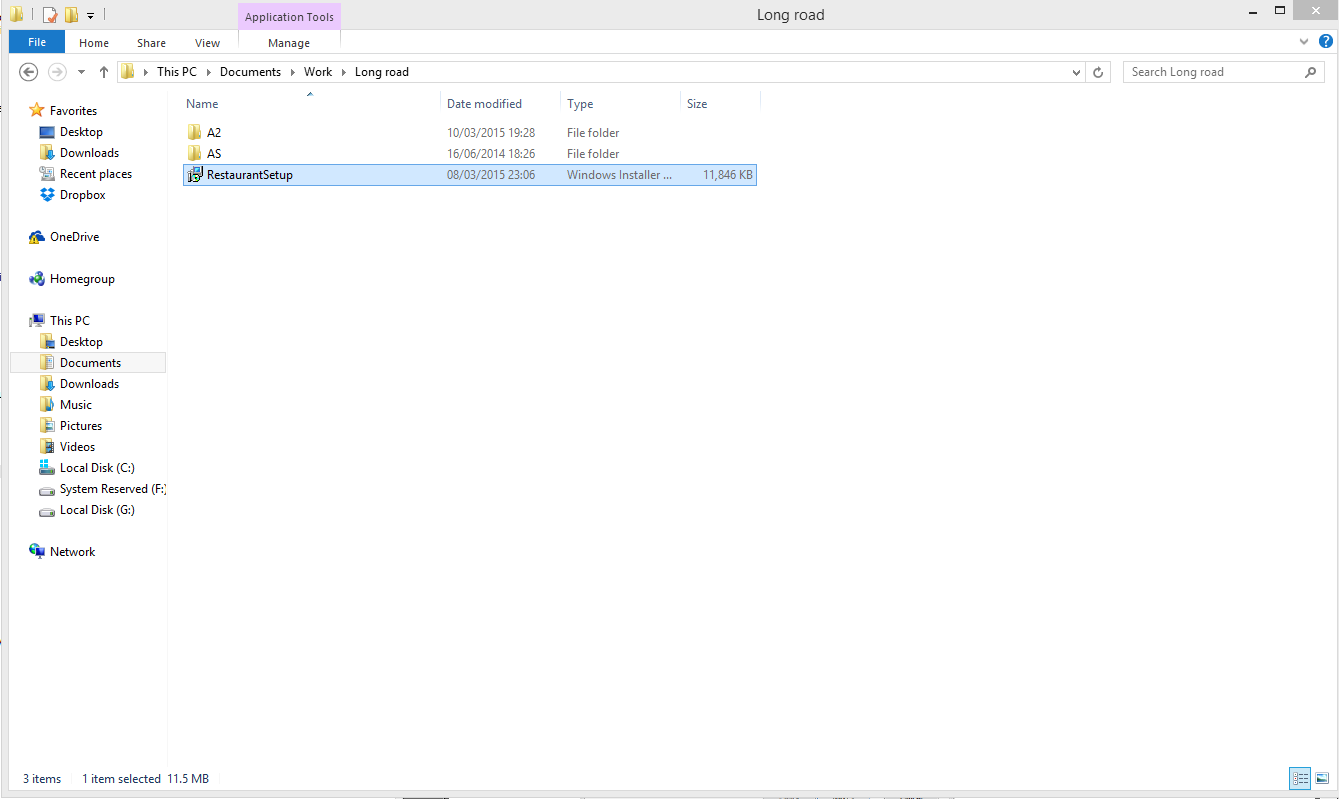
\includegraphics[height = 10cm]{./Manual/images/install1} 
    \caption{Example of what the installer should look like} \label{fig:install1}
\end{figure}


2. Double click on the installer to run it, the installer will now start to run.

\begin{figure}[H]
    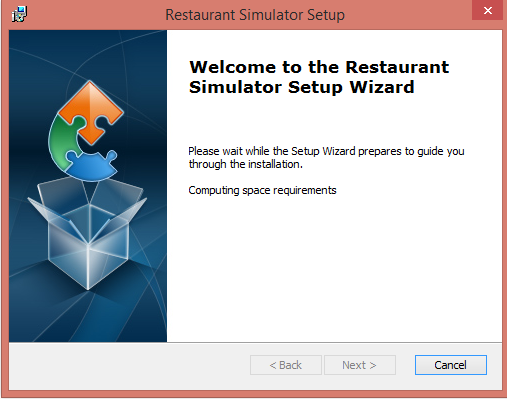
\includegraphics[height = 10cm]{./Manual/images/install2} 
    \caption{Start of the installer} \label{fig:install2}
\end{figure}

3. After waiting for the installer to prepare, the next step of the installer will appear and the step is to choose the directory(location) of where to install the new system.

\begin{figure}[H]
    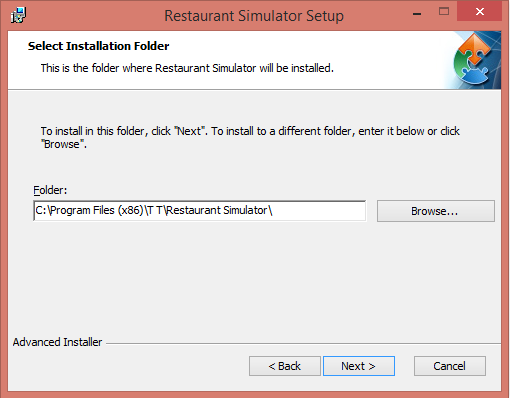
\includegraphics[height = 10cm]{./Manual/images/install3} 
    \caption{Choosing where to install the system} \label{fig:install3}
\end{figure}

4.  Click on 'Install' to start the installation

\begin{figure}[H]
    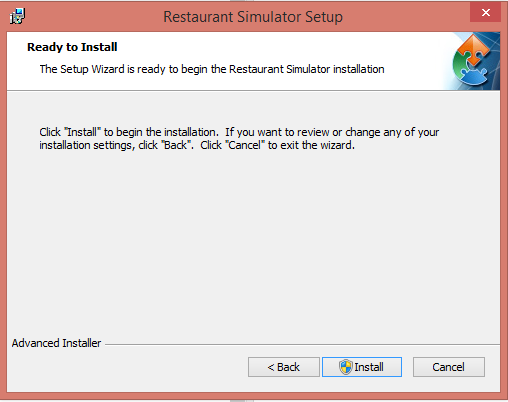
\includegraphics[height = 10cm]{./Manual/images/install4} 
    \caption{} \label{fig:install4}
\end{figure}

5. The installation will now begin, the installation will be complete once the status bar is filled.

\begin{figure}[H]
    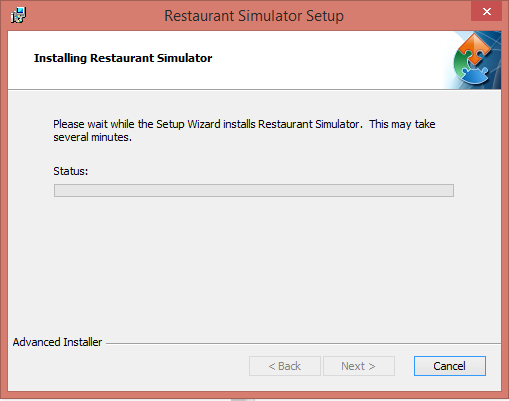
\includegraphics[height = 10cm]{./Manual/images/install5} 
    \caption{Install process} \label{fig:install5}
\end{figure}

6. The system has now been installed! Click on 'Finish' to close the installation.

\begin{figure}[H]
    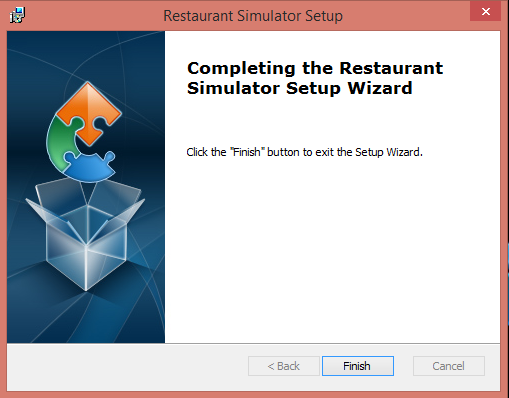
\includegraphics[height = 10cm]{./Manual/images/install6} 
    \caption{Successful installation} \label{fig:install6}
\end{figure}

7. As you can see, the system has been installed with all its necessary files. The application is called main\_window.

\begin{figure}[H]
    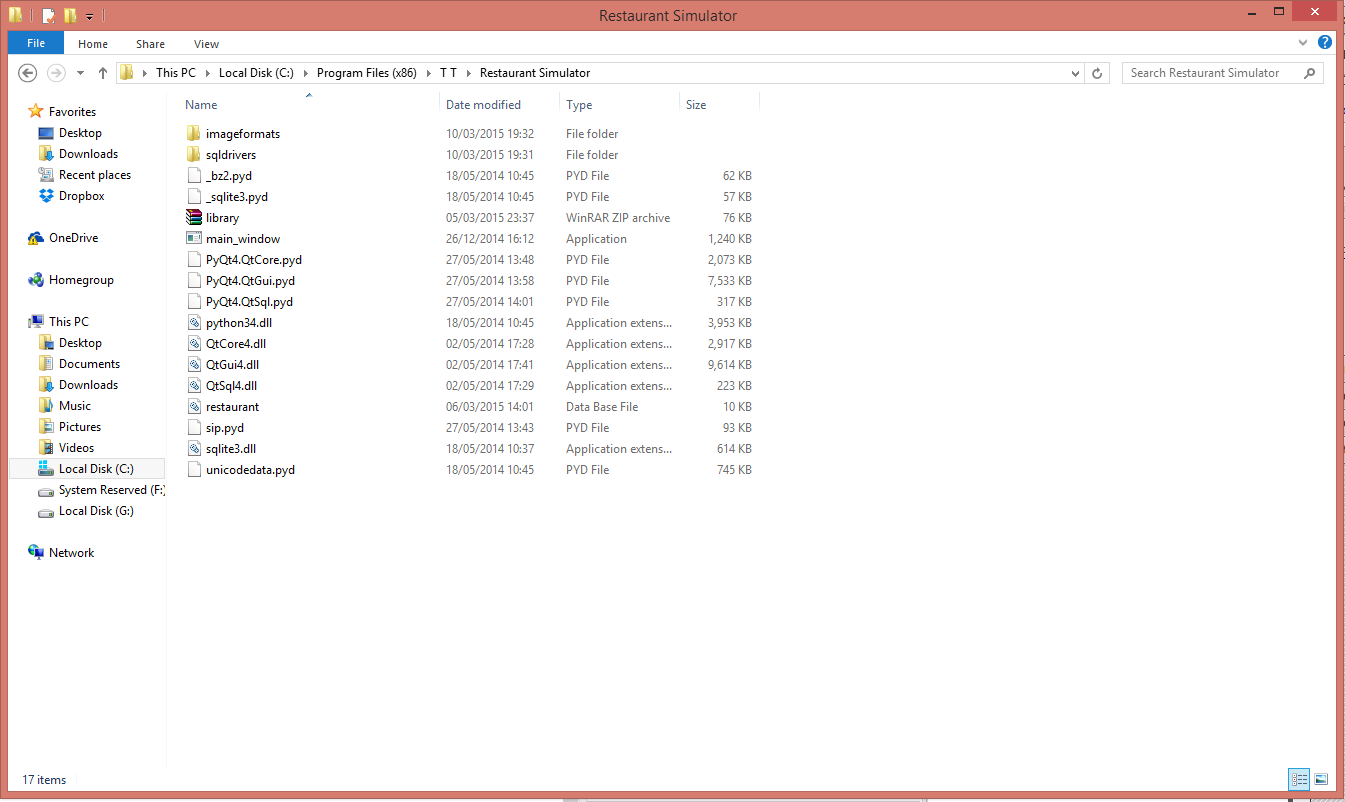
\includegraphics[height = 10cm]{./Manual/images/install7} 
    \caption{Installed system directory} \label{fig:install7}
\end{figure}


\subsection{Running the System}

1. To run the system, locate the directory of where you installed the system and locate the program called "main\_window". 

\begin{figure}[H]
    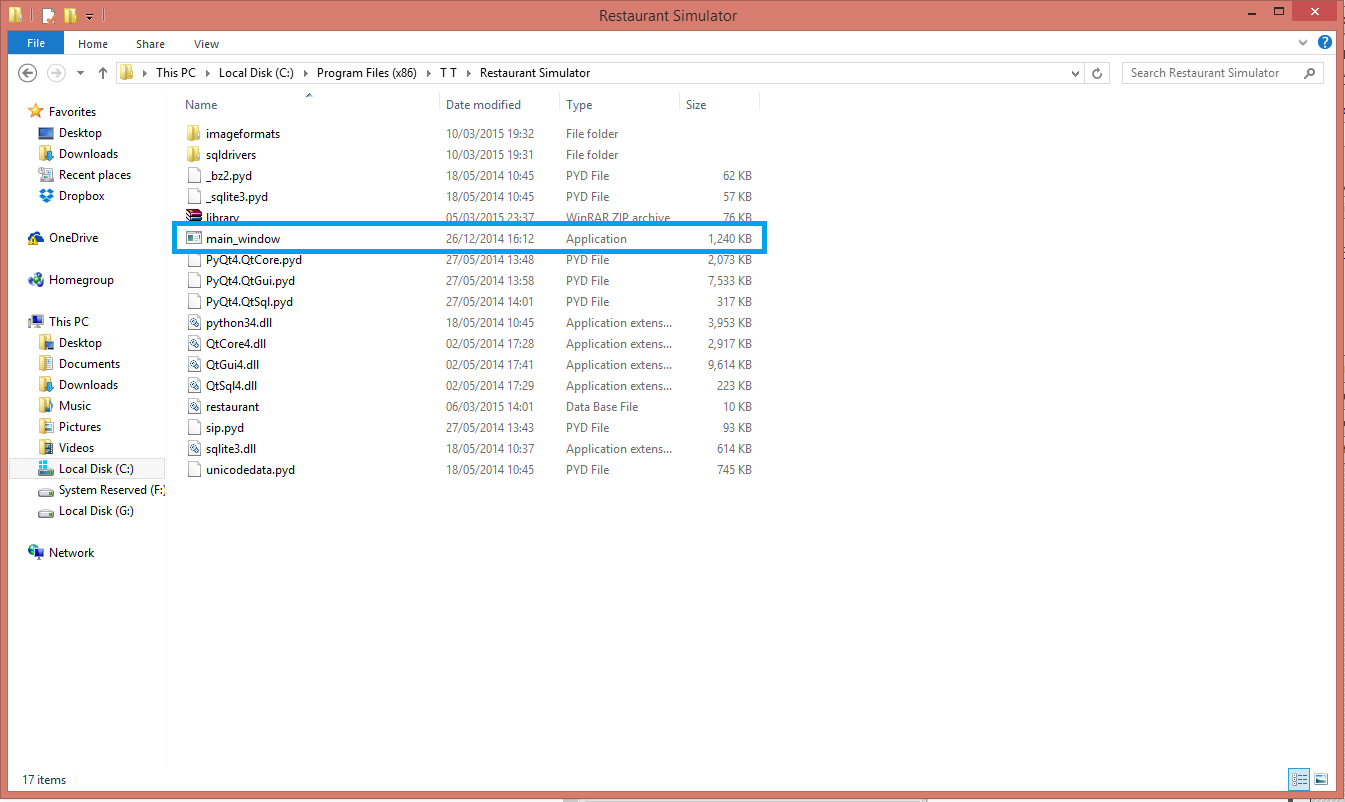
\includegraphics[height = 9cm]{./Manual/images/runsystem} 
    \caption{Locating the system program} \label{fig:locateSystem}
\end{figure}

2. Double click with the left mouse button on "main\_window" and the system should now run.

\begin{figure}[H]
    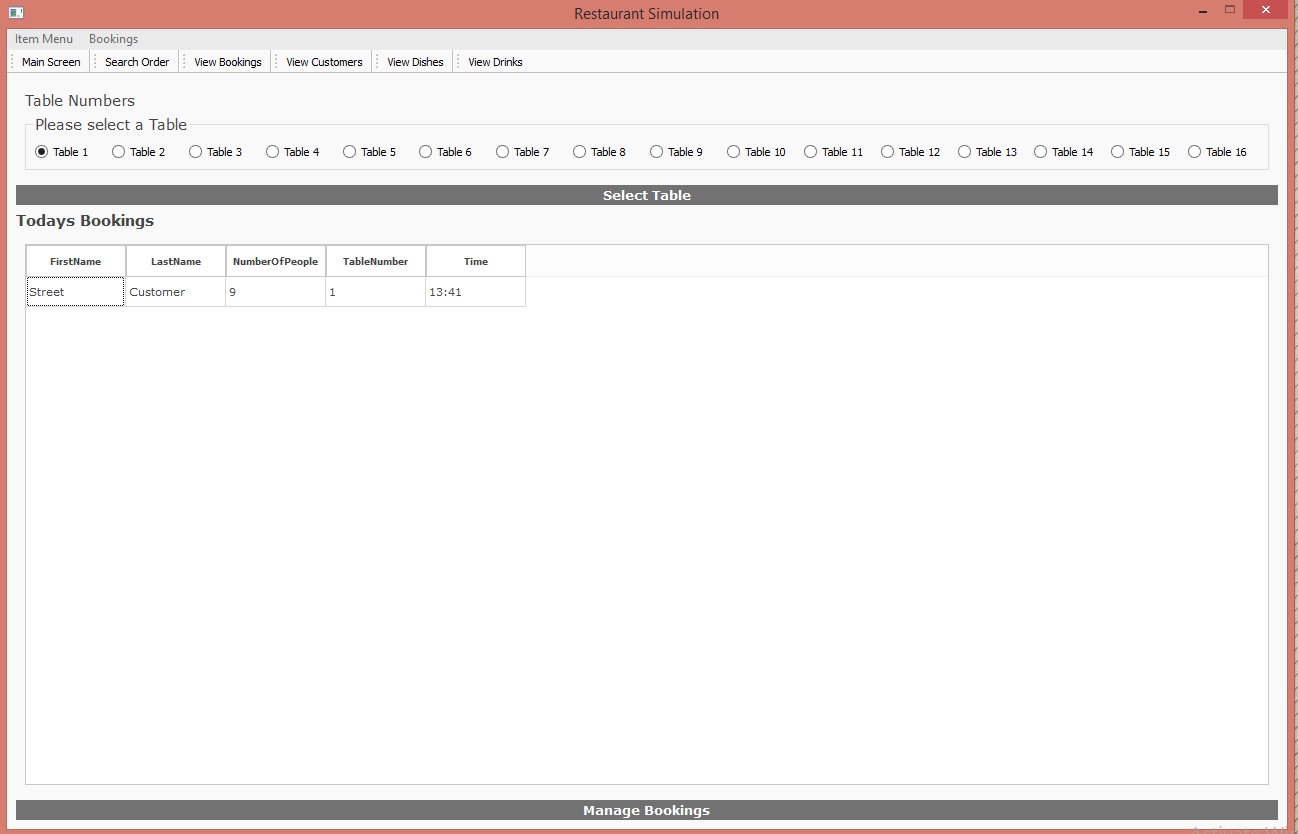
\includegraphics[height = 9cm]{./Testing/images/mainscreen} 
    \caption{Running the system} \label{fig:runSystem}
\end{figure}

Click on the big X at the top right to close the system.

\end{landscape}

\section{Tutorial}

\subsection{Introduction}

In this section, I will explain on how to use the system in depth by going through each feature of the system and giving instructions of what is required by the user to use the feature.

\subsection{Assumptions}

I have made assumptions that the user has little to no computer knowledge but does know how to use a keyboard, mouse and knows how to use the printer. Therefore, I will try to make the instructions as simple and clear as possible.

\subsection{Tutorial Questions}

\begin{center}
\begin{tabular}{|p{8cm}|p{2cm}|p{2cm}|}
    \hline
    \textbf{Question} & \textbf{Section} & \textbf{Page Number} \\ \hline
 How do I add an item to the menu? & 5.3.4 & \\ \hline
How do I delete an item off the menu? & 5.3.5 & \\ \hline
 How do I update an item's price?& 5.3.6 & \\ \hline
 How do I add a booking? & 5.3.7 & \\ \hline
 How do I delete a booking? & 5.3.8 & \\ \hline
 How do I update a booking? & 5.3.9 & \\ \hline
How do I manage an order for a table & 5.3.10 \\ \hline
 A customer has come in without booking advance, how do I assign him to a table? & 5.3.11 & \\ \hline
How do I add an item to the order? & 5.3.12& \\ \hline
 How do I delete an item off the order? & 5.3.13 & \\ \hline
 How do I print an invoice? & 5.3.14& \\ 

    \hline
\end{tabular}
\end{center}

\subsection{How do I add an item to the menu?}

1. Click on "Item Menu" at the top on the menu bar.
\begin{figure}[H]
    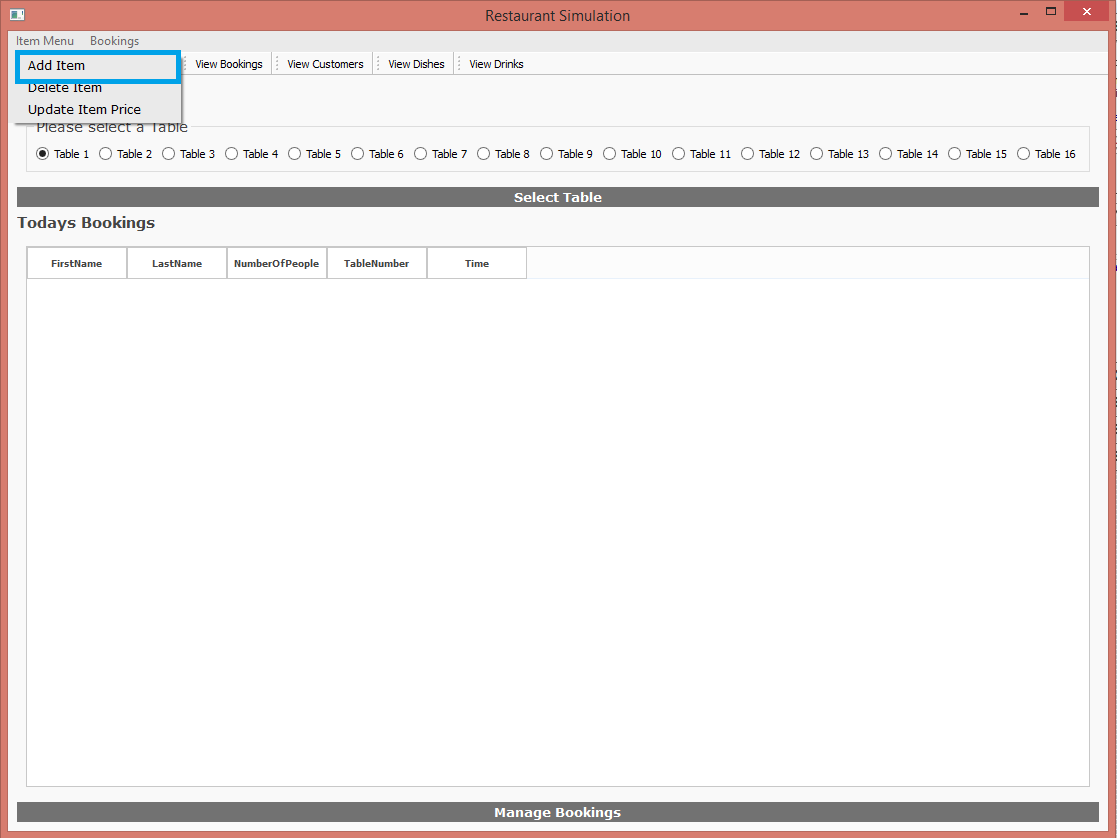
\includegraphics[height = 9cm]{./Manual/images/AddItem1} 
    \caption{} \label{fig:additem1}
\end{figure}

2. Click on "Add Item" and the add item screen should appear.

3. Fill in the fields at the bottom where the first field is for the item name, the second for the price and the third is a drop down where you would have to select what item type it is

\begin{figure}[H]
    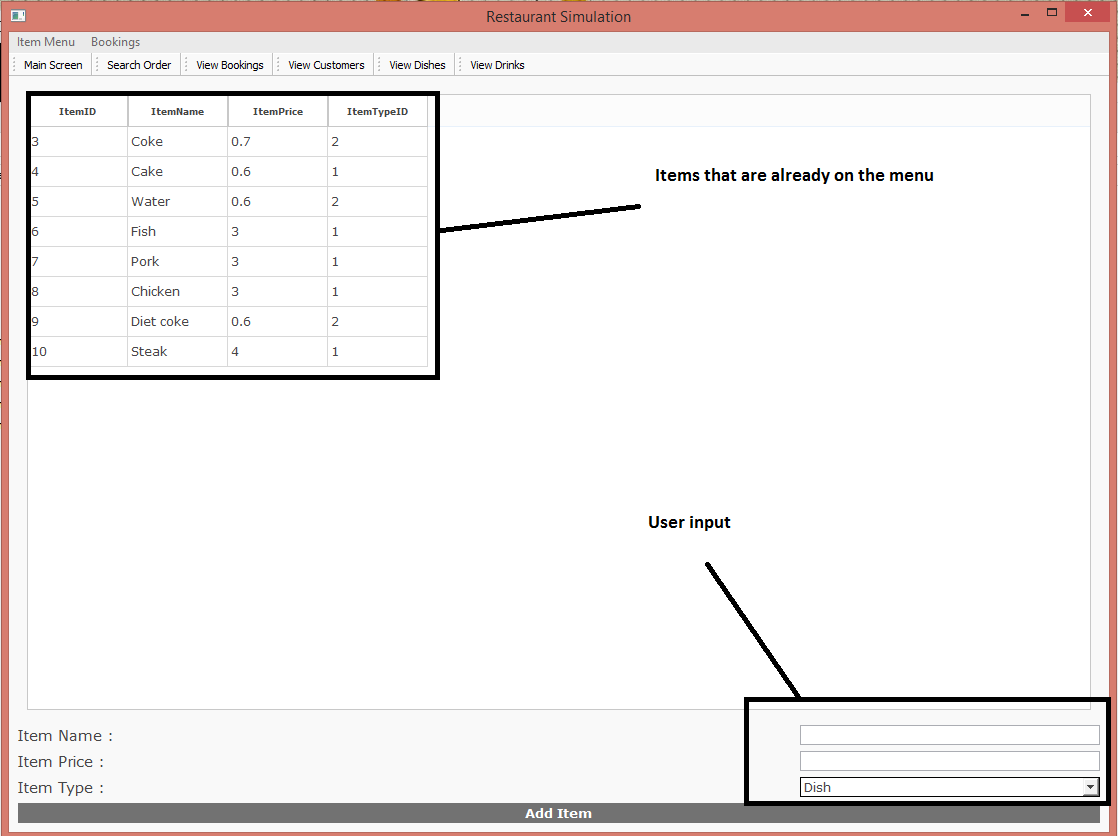
\includegraphics[height = 9cm]{./Manual/images/AddItem2} 
    \caption{} \label{fig:additem2}
\end{figure}

\begin{figure}[H]
    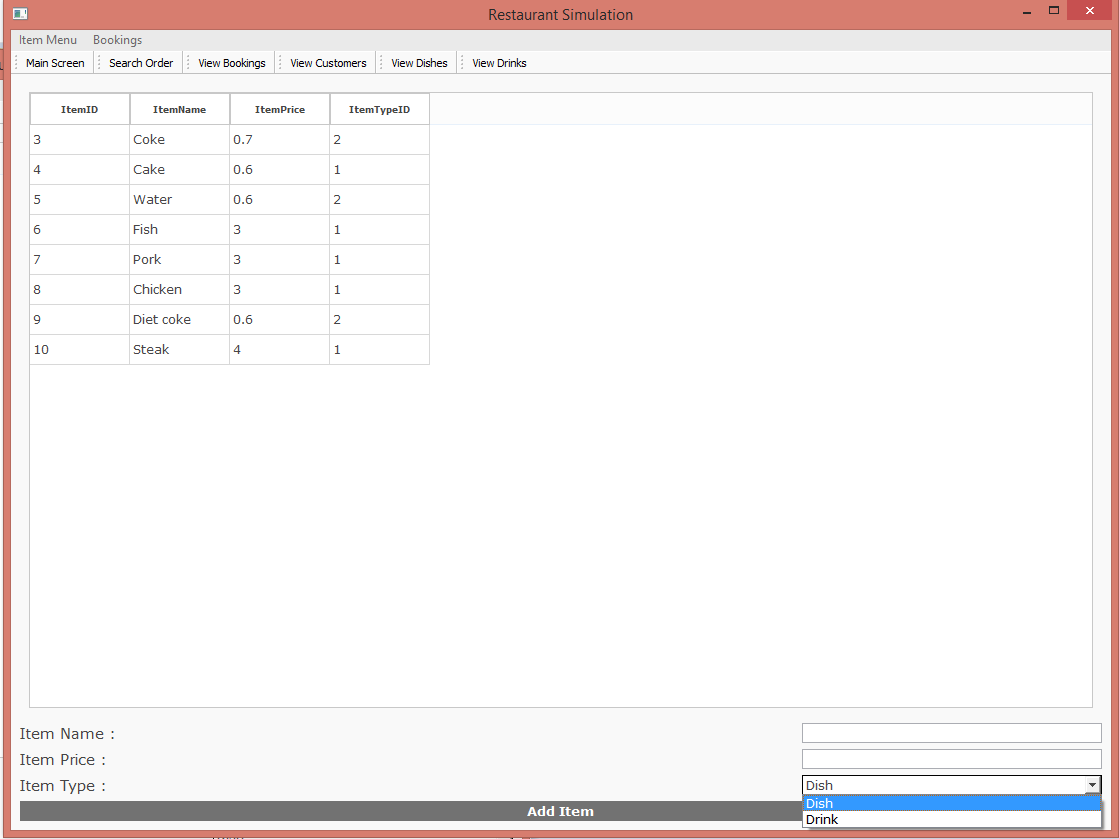
\includegraphics[height = 9cm]{./Manual/images/AddItem3} 
    \caption{} \label{fig:additem3}
\end{figure}

4. Click on Add Item after filling in the fields and the item should appear in the table above.

\subsection{How do I delete an item off the menu?}
1. Click on Item Menu at the top on the menu bar.

2. Click on "Delete Item" and the delete item screen should appear as shown in the image below.

\begin{figure}[H]
    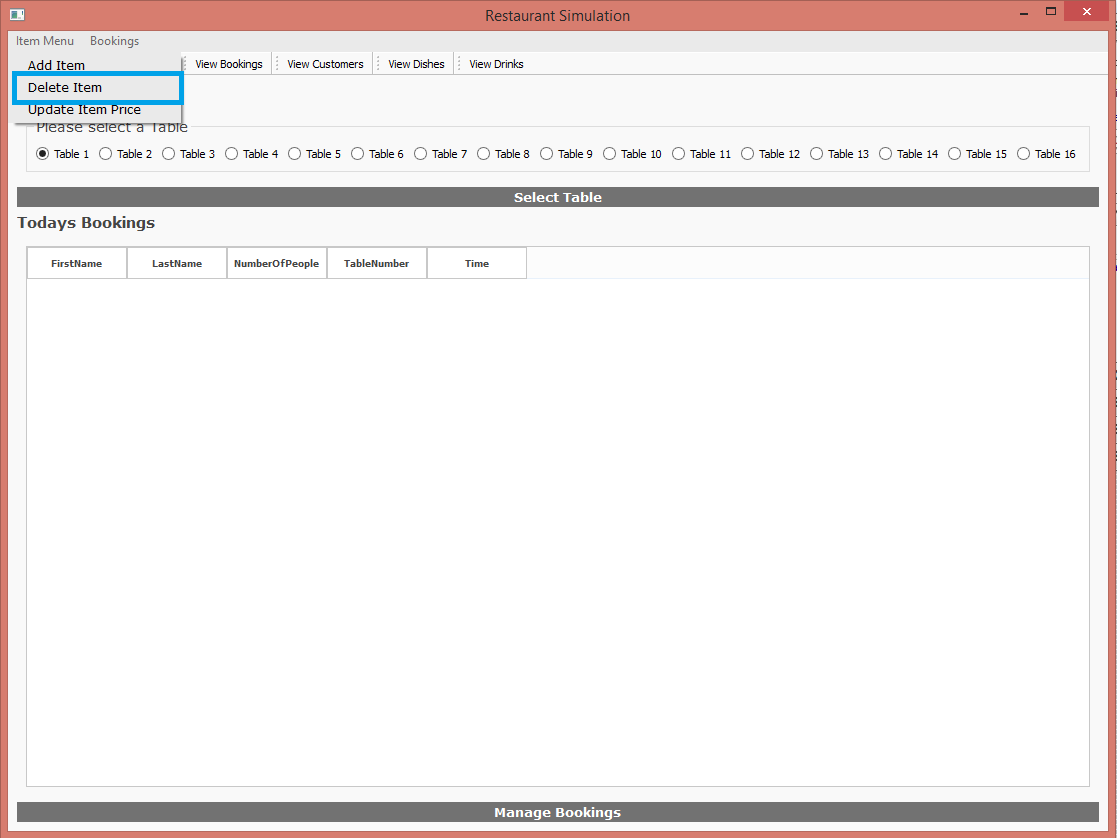
\includegraphics[height = 9cm]{./Manual/images/DeleteItem1} 
    \caption{} \label{fig:deleteitem1}
\end{figure}

3.  You can either delete an item by inputting the item name or its ID at the respective fields. The first field is for the Item Name and the second is for the ID. You would also have to click on the correct 'Delete Item' button - first button( same row as item name) is for the item name and second is for the id.

\begin{figure}[H]
    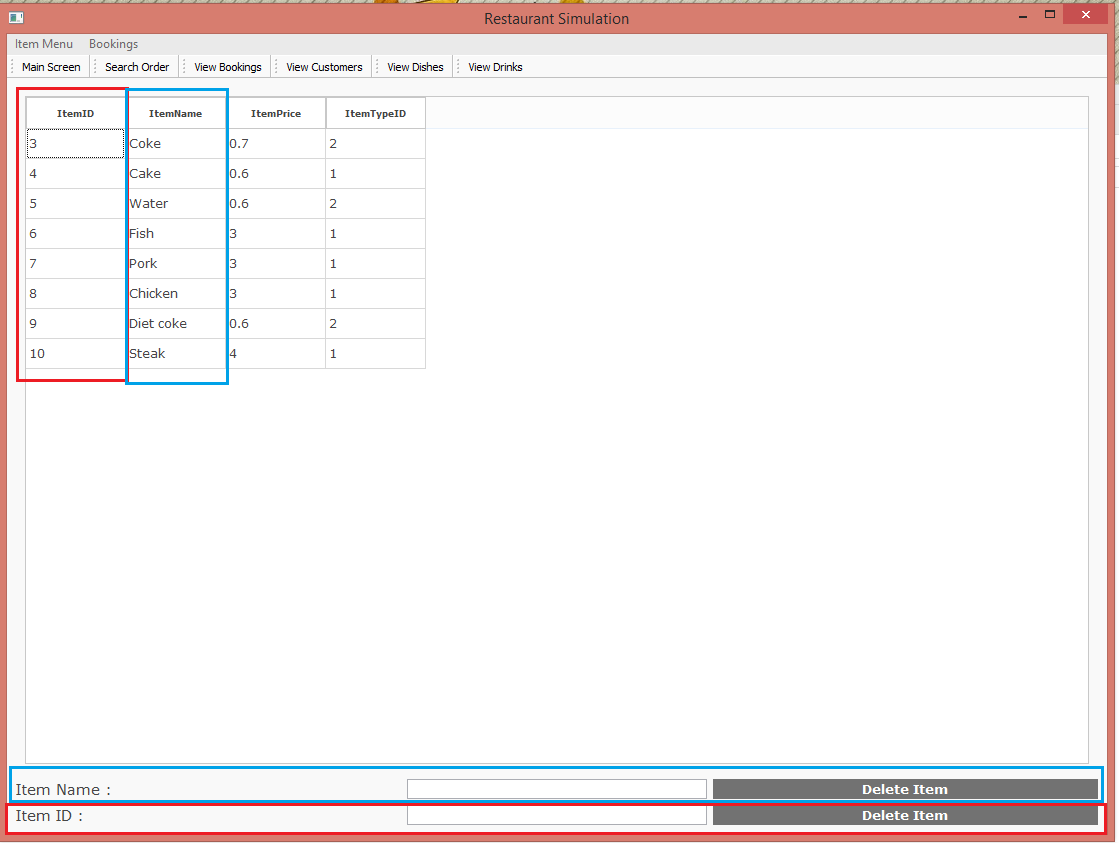
\includegraphics[height = 9cm]{./Manual/images/DeleteItem2} 
    \caption{} \label{fig:deleteitem2}
\end{figure}

4. The item will delete if you successfully fill in the field. The item will be deleted from the table above the fields.

\subsection{How do I update an item's price?}
1. Click on "Item Menu" at the top on the menu bar

2 Click on "Update Item Price" and the  update item screen should appear as shown in the image below.
\begin{figure}[H]
    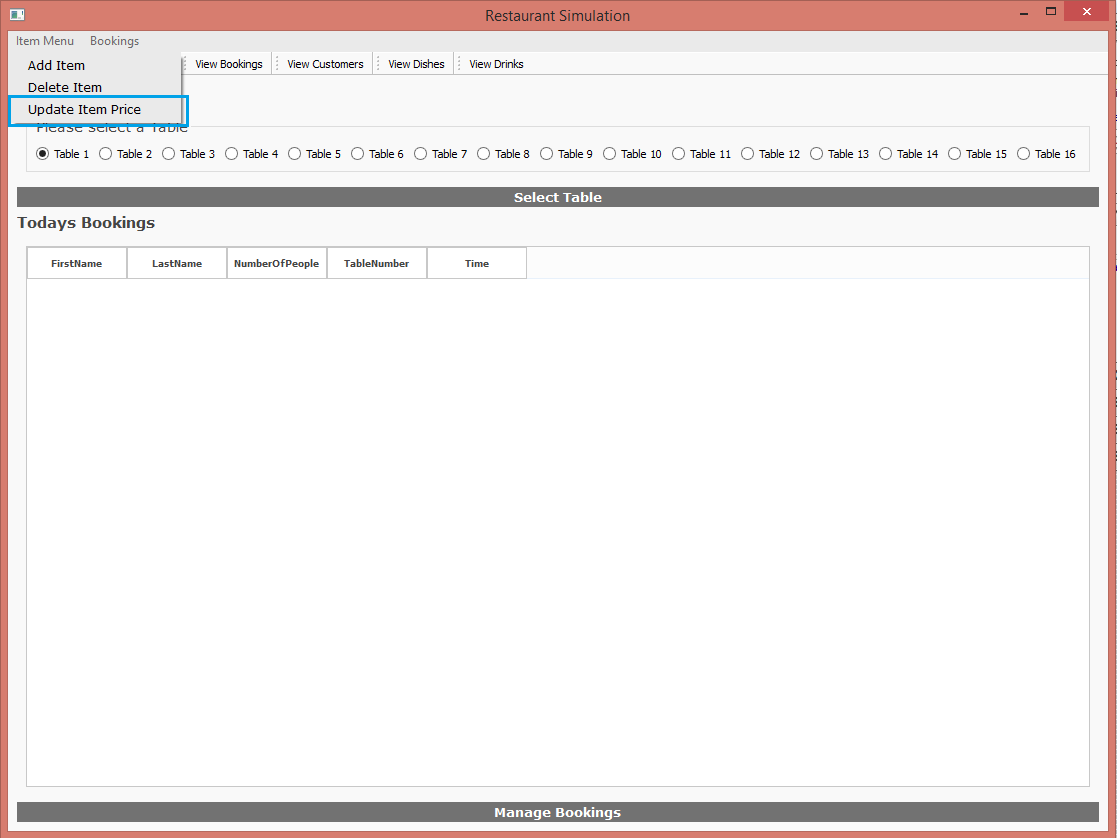
\includegraphics[height = 9cm]{./Manual/images/UpdateItem1} 
    \caption{} \label{fig:updateitem1}
\end{figure}

3. Use the table above to assist you on what item you wish to update.

4. Fill in the fields - first field is for the item ID and second is for the price you wish to change it to

5. Click on "Update Item"
\begin{figure}[H]
    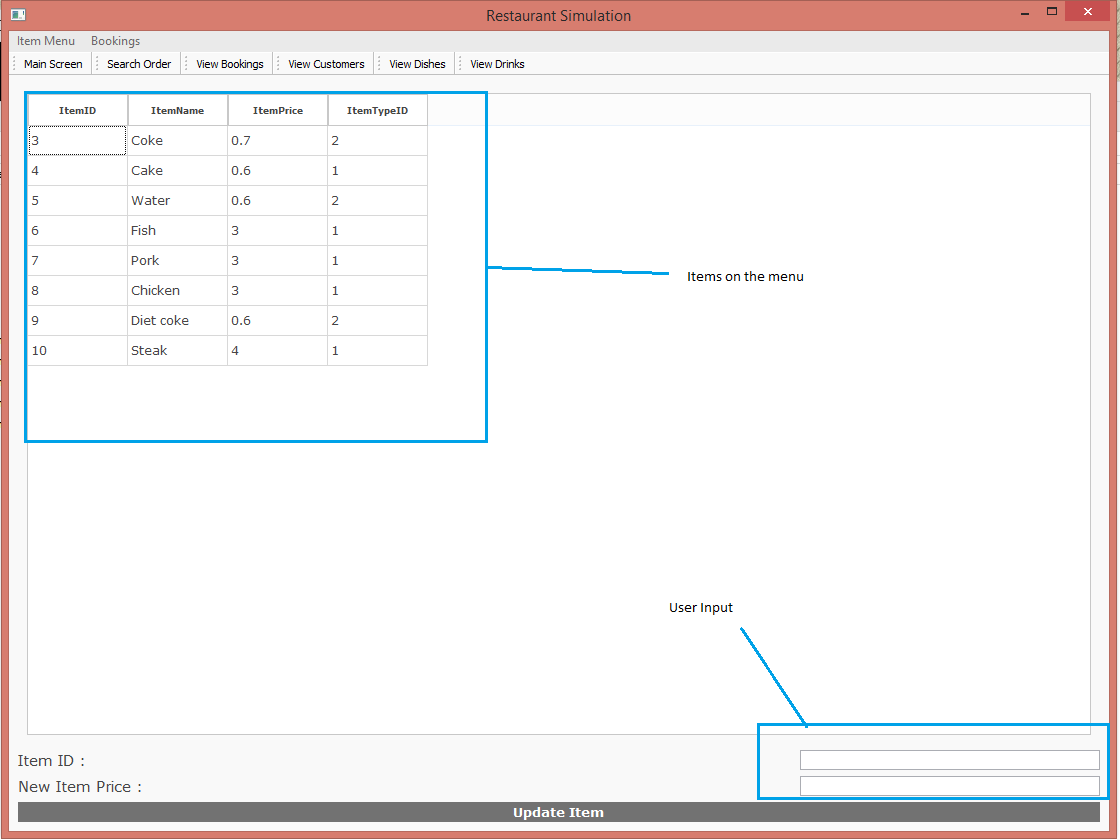
\includegraphics[height = 9cm]{./Manual/images/UpdateItem2} 
    \caption{} \label{fig:updateitem2}
\end{figure}

6. The item should successfully update - you can check with the item table above.

\subsection{How do I add a booking?}
1. Click on "Bookings" at the top on the menu bar

2. Click on "Add Booking" and the add booking screen should appear as shown in the image below.
%\subsubsection{Using the menu bar}

\begin{figure}[H]
    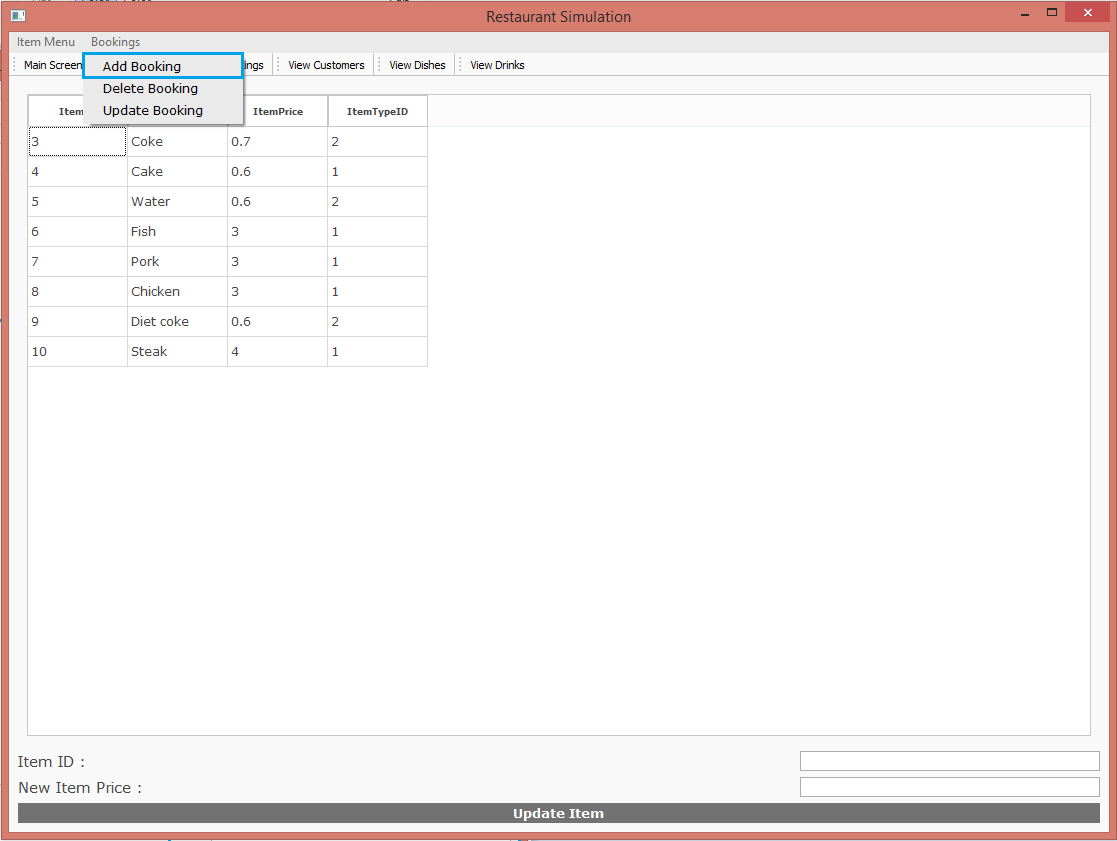
\includegraphics[height = 9cm]{./Manual/images/AddBooking1} 
    \caption{} \label{fig:addbooking1}
\end{figure}

3. As you can see in the image below, you would have to fill in the required fields where I have boxed and labeled 'User Input'.

\begin{figure}[H]
    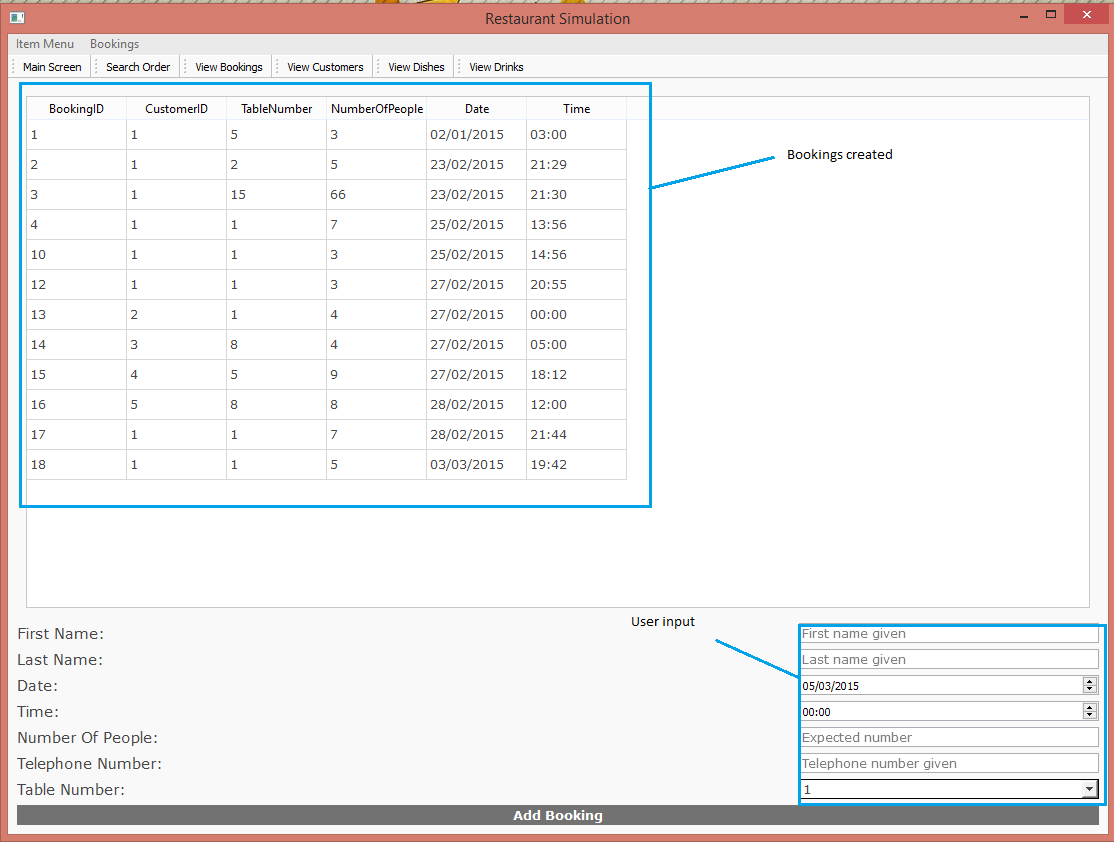
\includegraphics[height = 9cm]{./Manual/images/AddBooking2} 
    \caption{} \label{fig:addbooking2}
\end{figure}

The table number field is a drop down box which has 16 numbers as there are 16 tables.

\begin{figure}[H]
    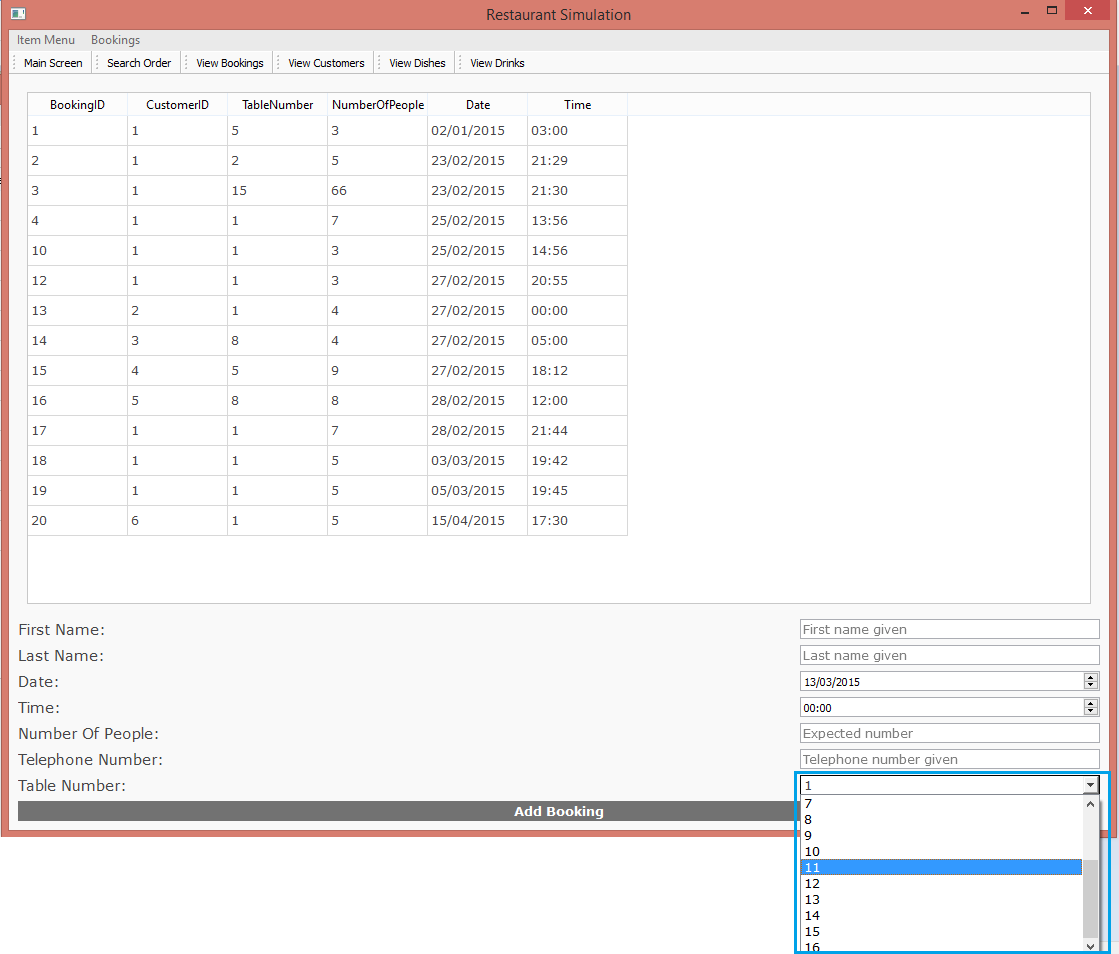
\includegraphics[height = 9cm]{./Manual/images/AddBooking3} 
    \caption{} \label{fig:addbooking3}
\end{figure}

4. Click on "Add Booking" .

5. The booking should appear in the table above if it has been created successfully.

\subsection{How do I delete a booking?}

%\subsubsection{Using the menu bar}

\begin{figure}[H]
    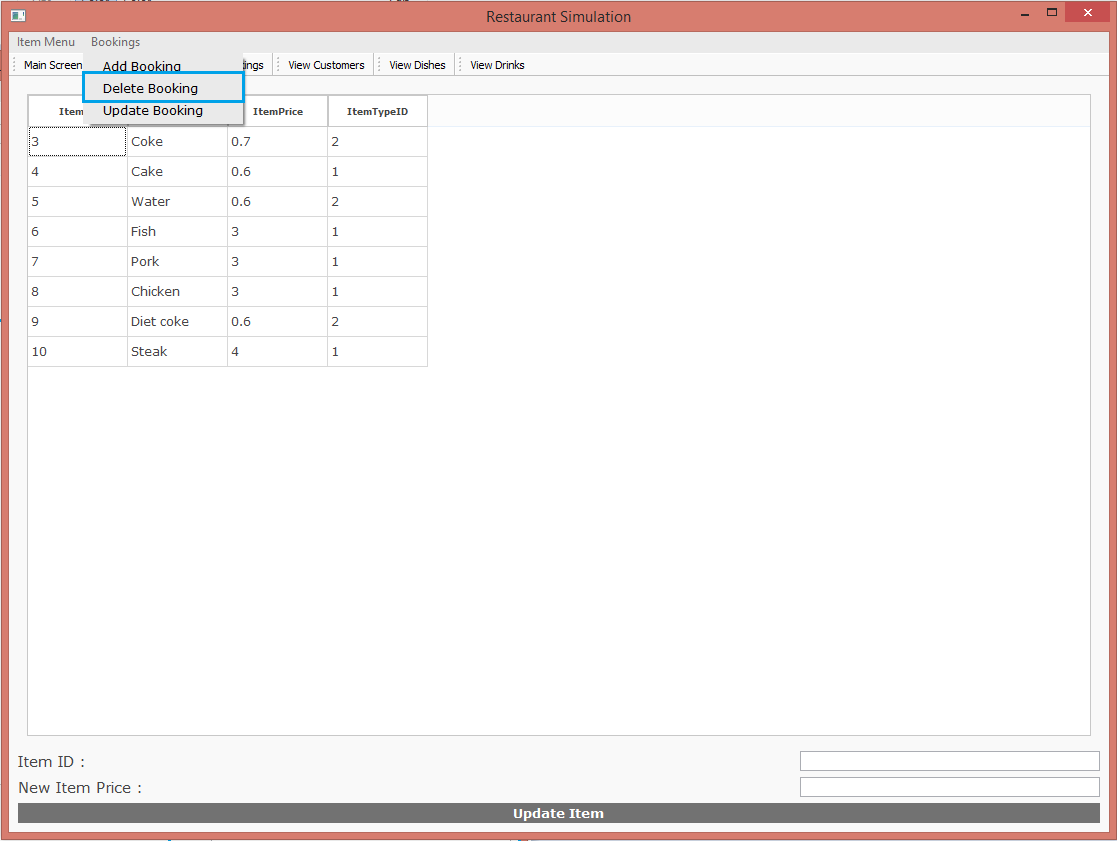
\includegraphics[height = 9cm]{./Manual/images/DeleteBooking1} 
    \caption{} \label{fig:deletebooking1}
\end{figure}

\begin{figure}[H]
    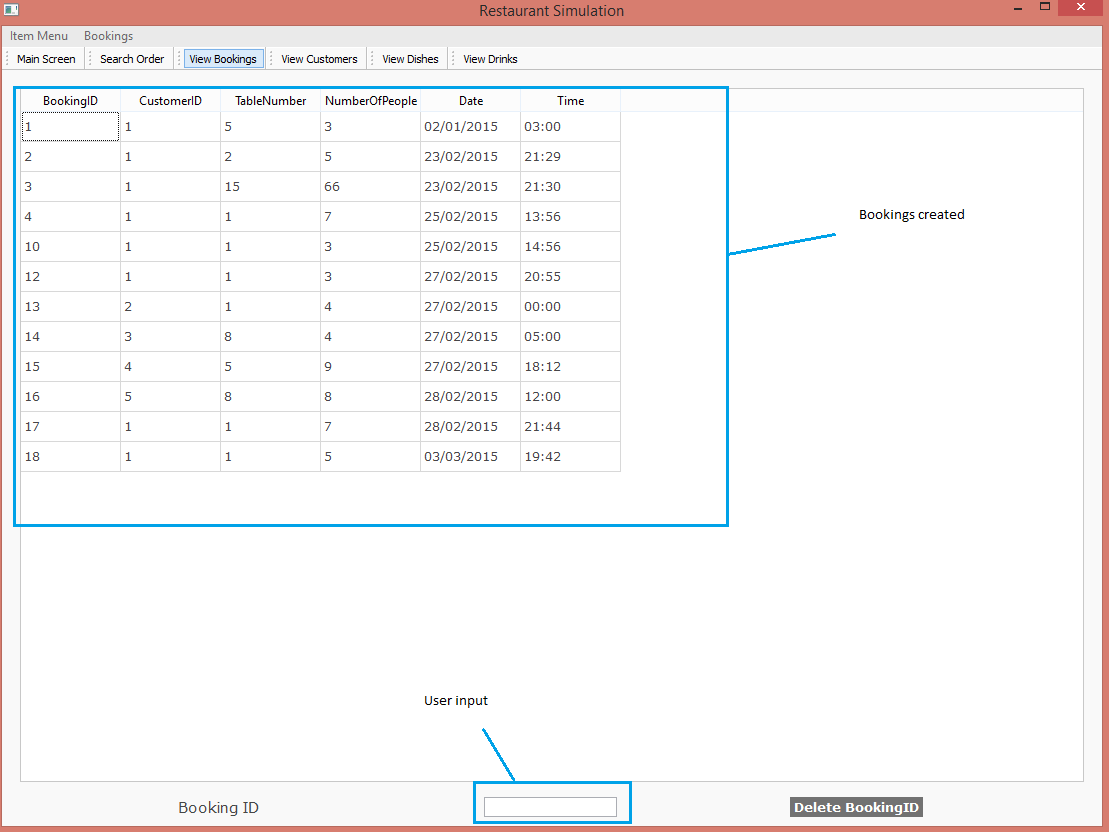
\includegraphics[height = 9cm]{./Manual/images/DeleteBooking2} 
    \caption{} \label{fig:deletebooking2}
\end{figure}

\subsection{How do I update a booking?}

\begin{figure}[H]
    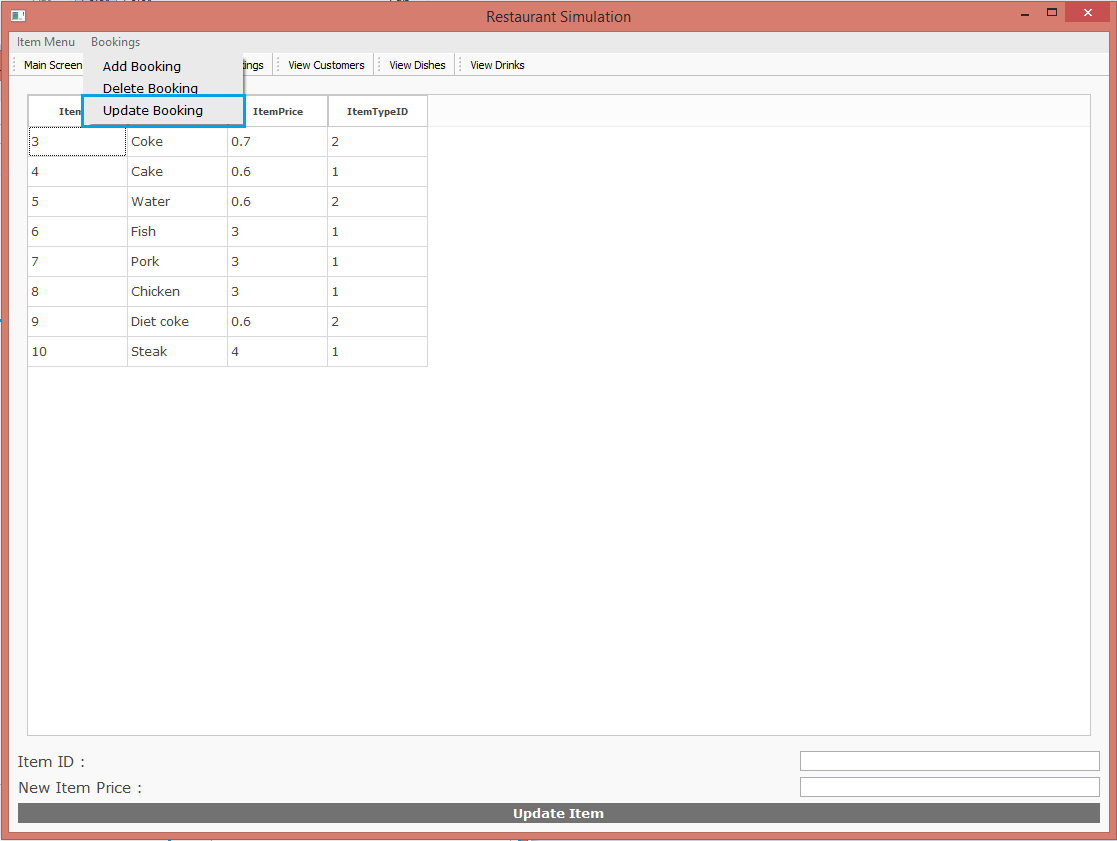
\includegraphics[height = 9cm]{./Manual/images/UpdateBooking1} 
    \caption{} \label{fig:updatebooking1}
\end{figure}

\begin{figure}[H]
    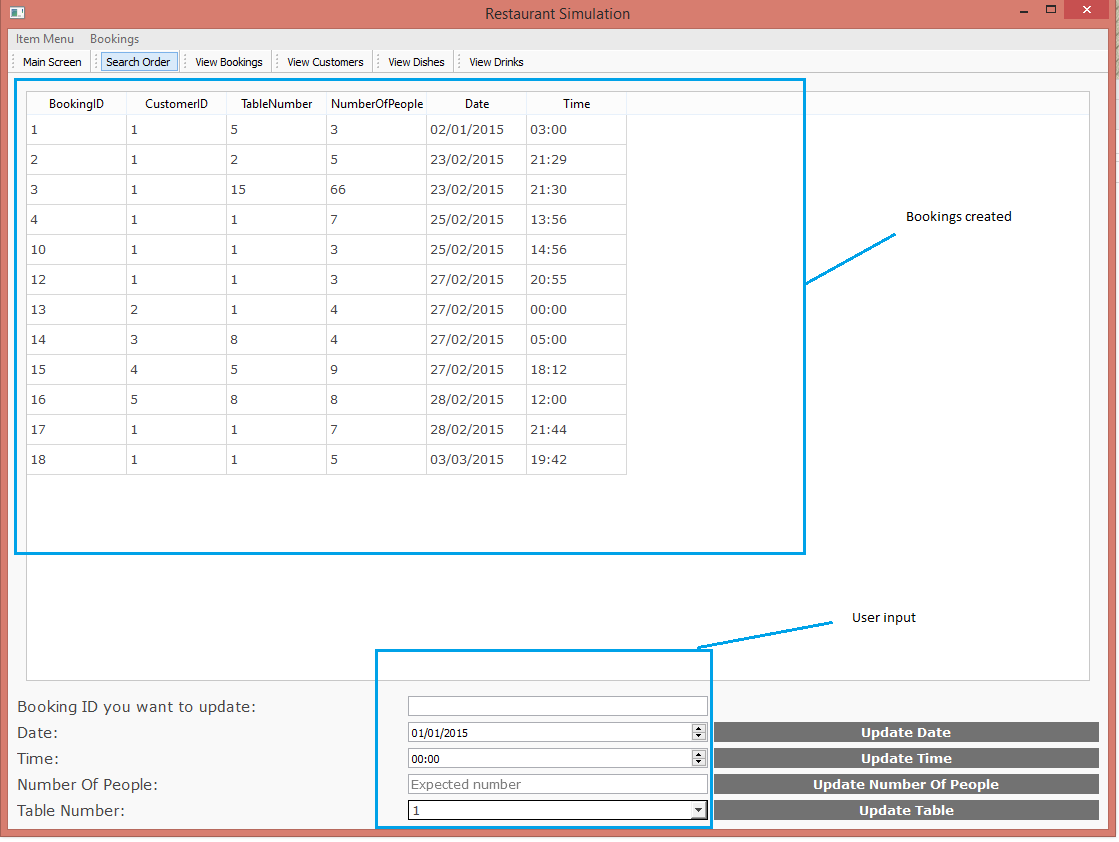
\includegraphics[height = 9cm]{./Manual/images/UpdateBooking2} 
    \caption{} \label{fig:updatebooking2}
\end{figure}

\subsection{How do I manage an order for a table?}
First of all, you have to assign the customer to the table. Assuming the customer has booked in advance, follow these steps:

1. Click on the selected table that has been booked ( My example will be on table 1).

2. Make sure that the correct customer has been selected. The last names will be displayed in the drop down box as shown below (Only 1 customer in my example).
\begin{figure}[H]
    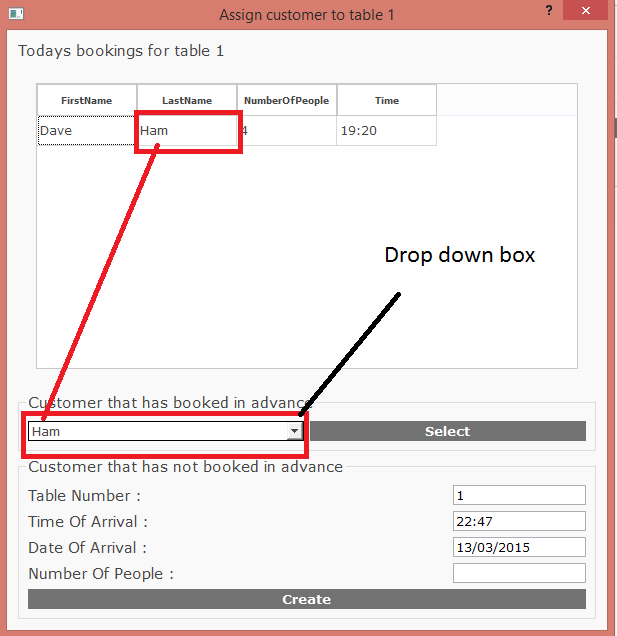
\includegraphics[height = 9cm]{./Manual/images/assignExample1} 
    \caption{} \label{fig:assignex1}
\end{figure}

3. Click on "Select" beside the drop down box

\begin{figure}[H]
    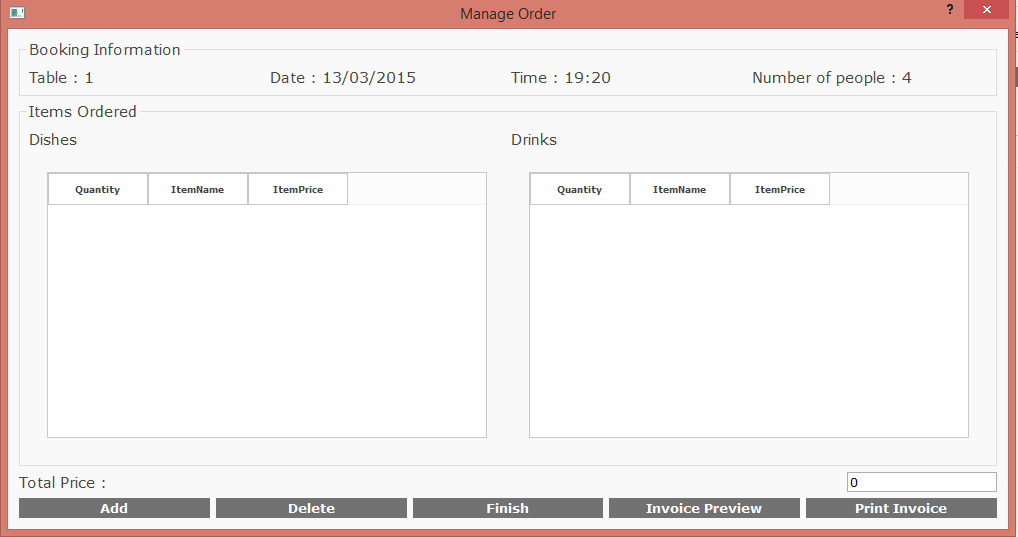
\includegraphics[height = 9cm]{./Manual/images/base/assignExample2} 
    \caption{} \label{fig:assignex2}
\end{figure}

\subsection{A customer has come in without booking in advance how do I assign him to a table?}
Assuming a group of customers wanted to come in and you wanted to assign them to table 1.

\begin{figure}[H]
    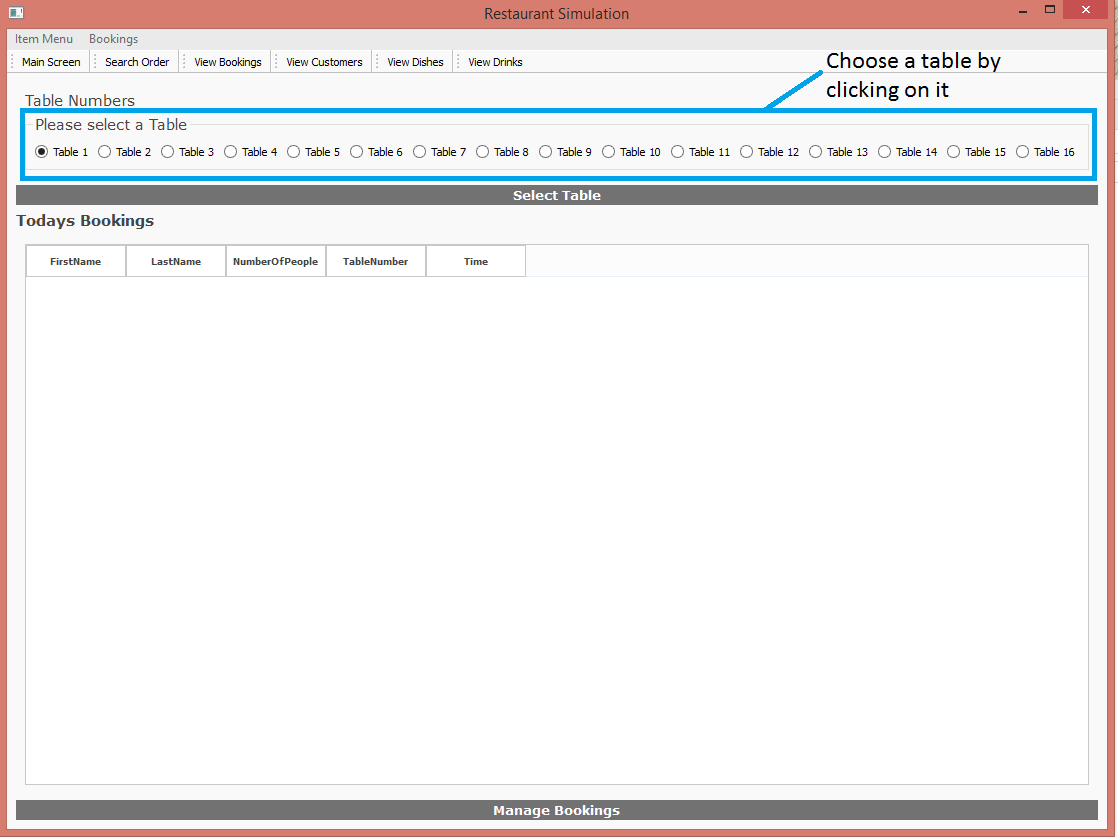
\includegraphics[height = 9cm]{./Manual/images/AssignCust1} 
    \caption{} \label{fig:assigncust1}
\end{figure}

\begin{figure}[H]
    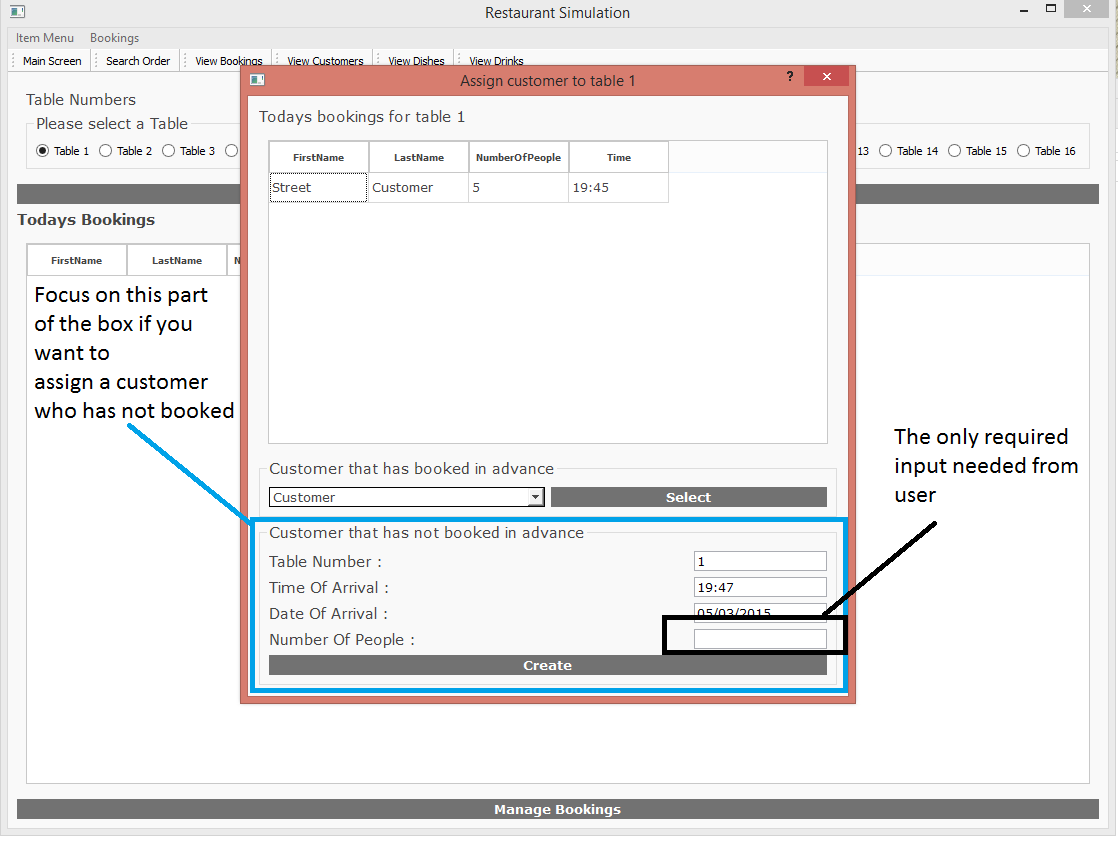
\includegraphics[height = 9cm]{./Manual/images/AssignCust2} 
    \caption{} \label{fig:assigncust2}
\end{figure}

\begin{figure}[H]
    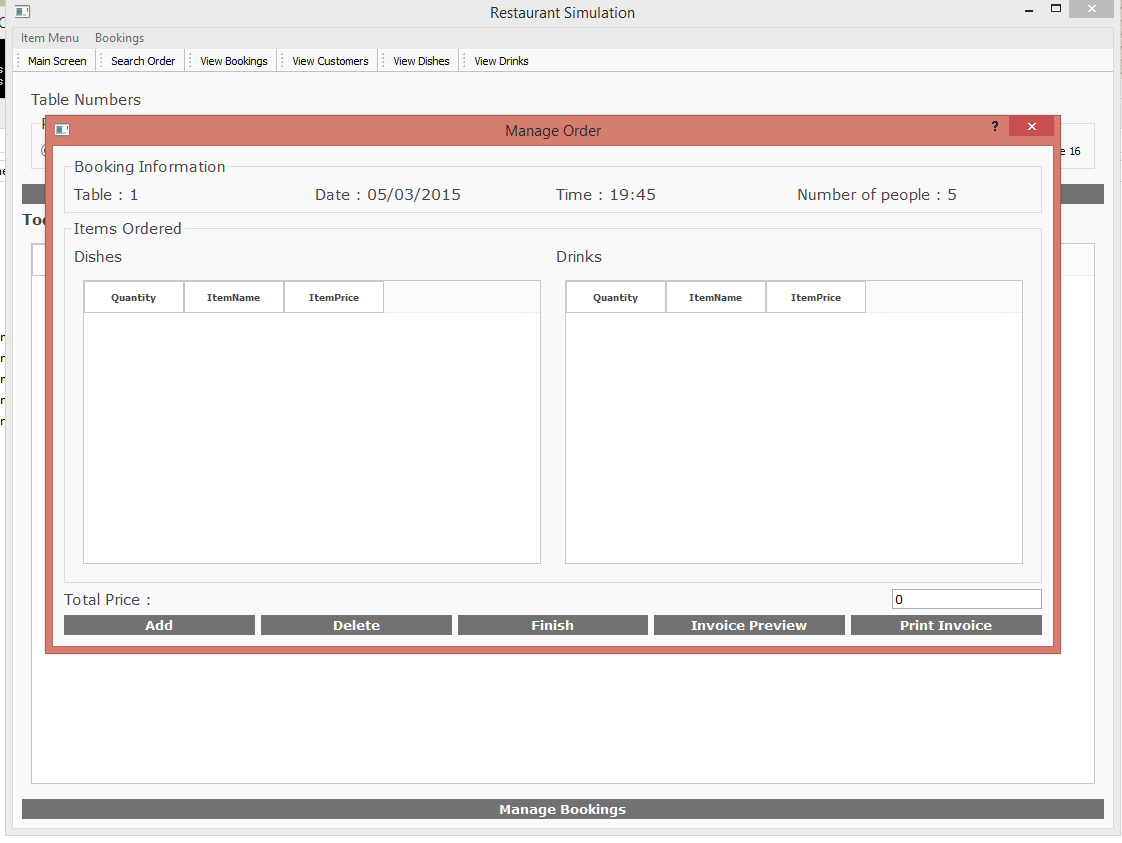
\includegraphics[height = 9cm]{./Manual/images/base/ManageOrder} 
    \caption{} \label{fig:assigncust3}
\end{figure}

\subsection{How do I add an item to an order}

1. Go to the selected table's manage order box by selecting the table and clicking on 'Select Table' at the main screen.

\begin{figure}[H]
    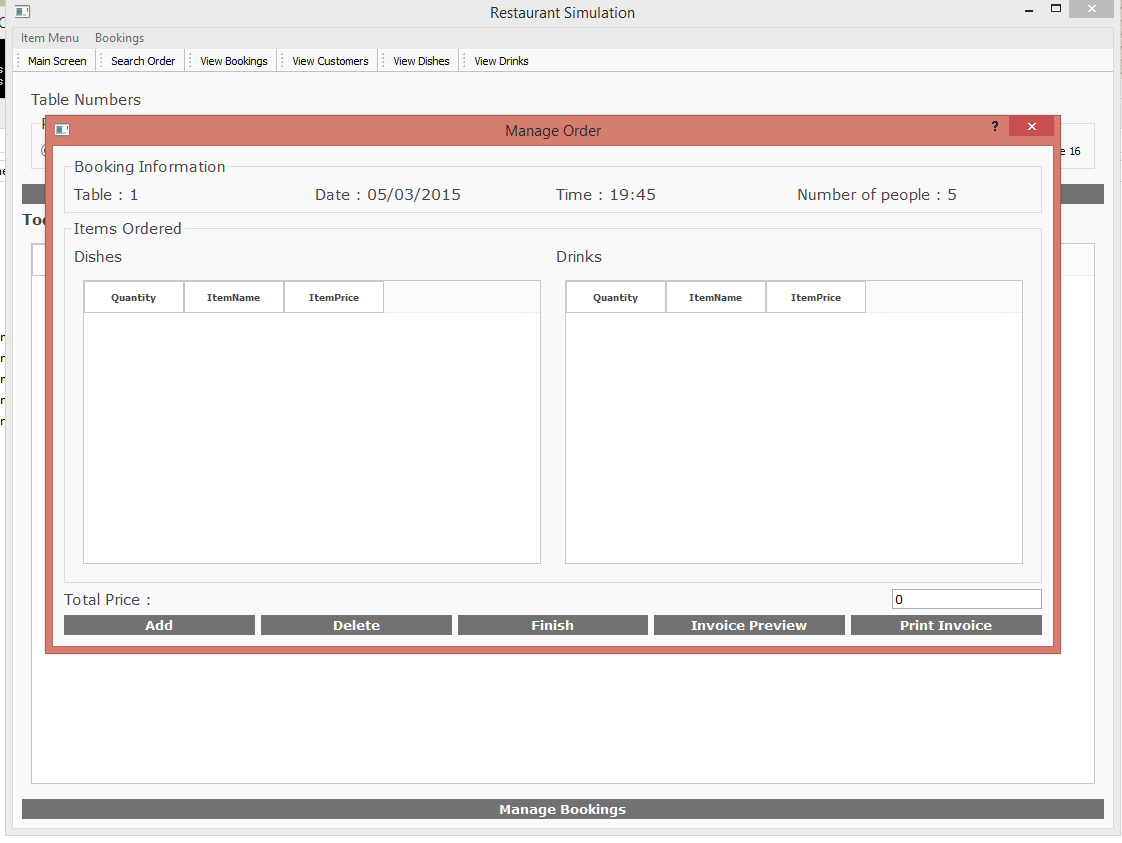
\includegraphics[height = 9cm]{./Manual/images/base/ManageOrder} 
    \caption{} \label{fig:additemorder1}
\end{figure}

2. Click on 'Add'

\begin{figure}[H]
    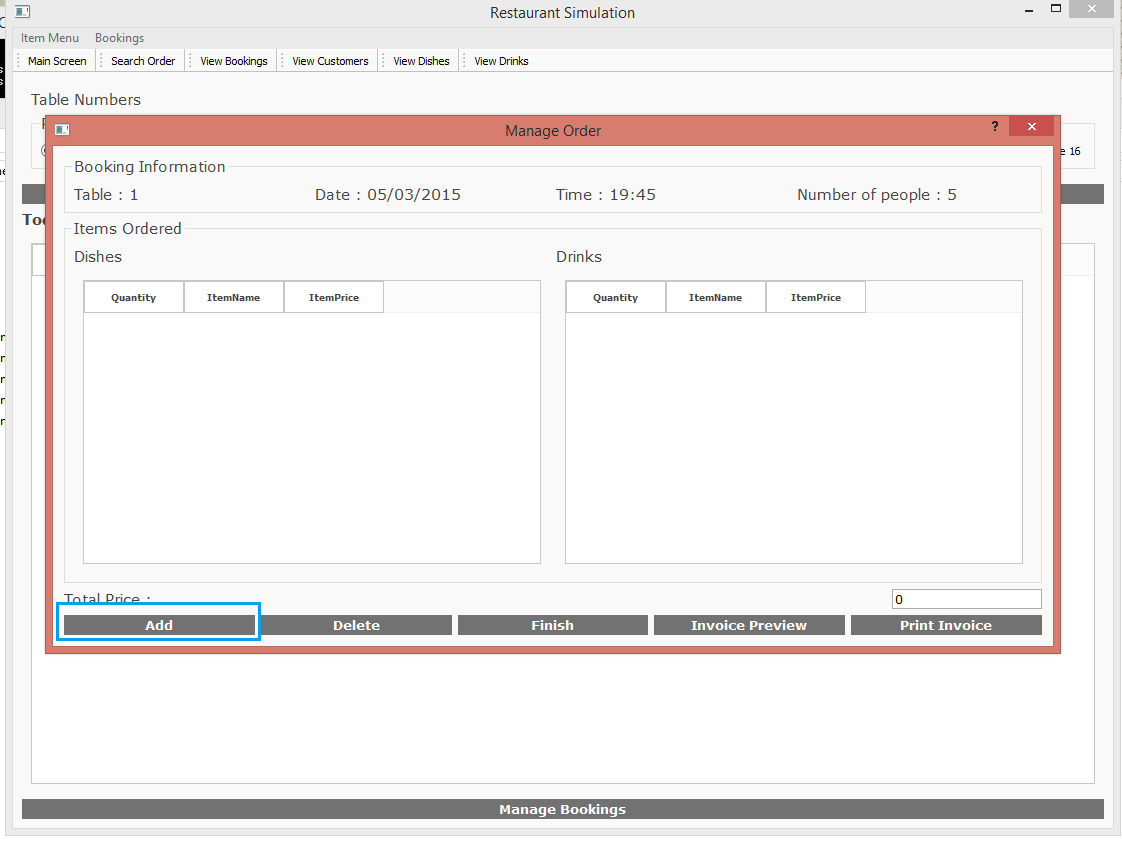
\includegraphics[height = 9cm]{./Manual/images/AddItemOrder1} 
    \caption{} \label{fig:additemorder2}
\end{figure}

\begin{figure}[H]
    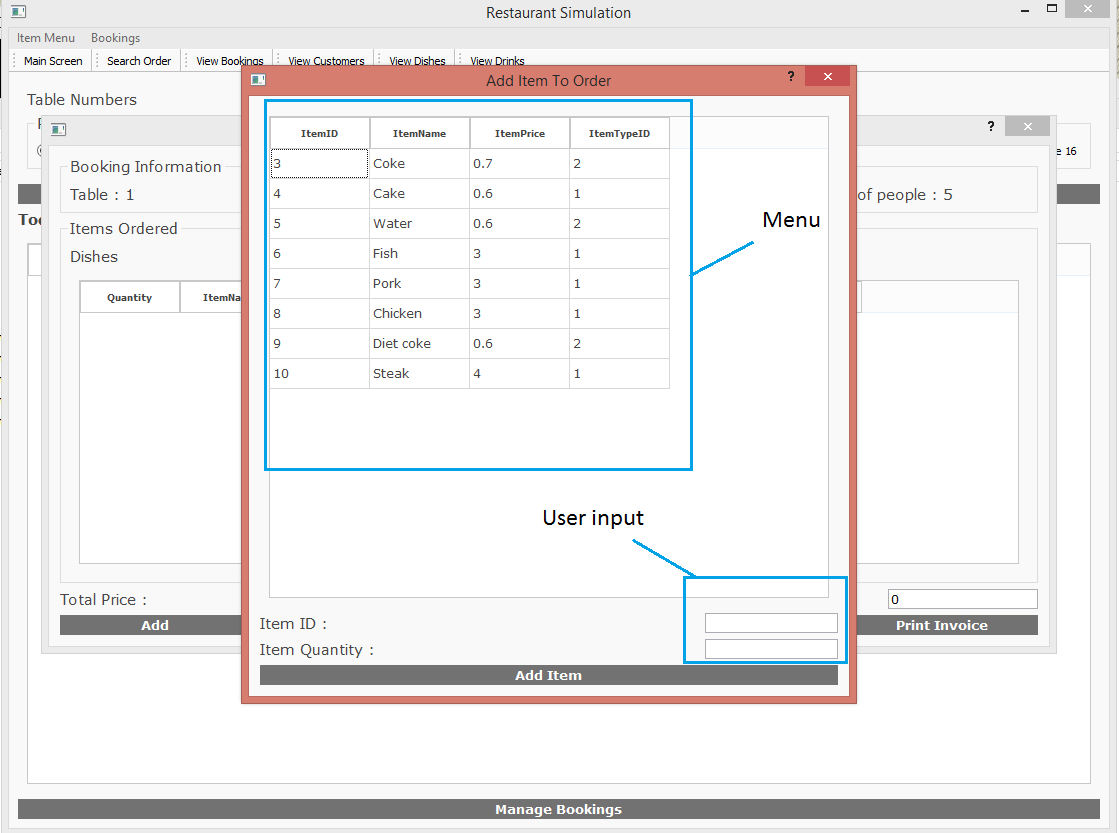
\includegraphics[height = 9cm]{./Manual/images/AddItemOrder2} 
    \caption{} \label{fig:additemorder3}
\end{figure}

\subsection{How do I delete an item off an order}

\begin{figure}[H]
    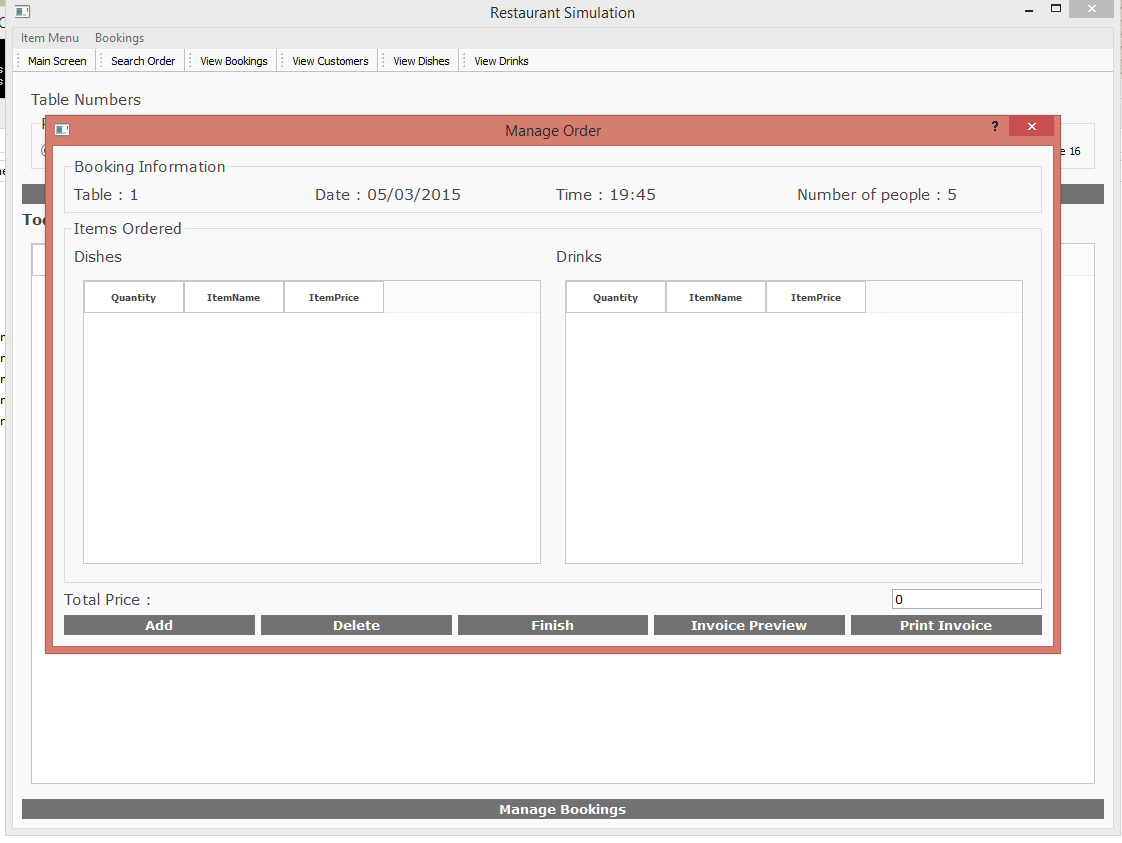
\includegraphics[height = 9cm]{./Manual/images/base/ManageOrder} 
    \caption{} \label{fig:additemorder1}
\end{figure}

\begin{figure}[H]
    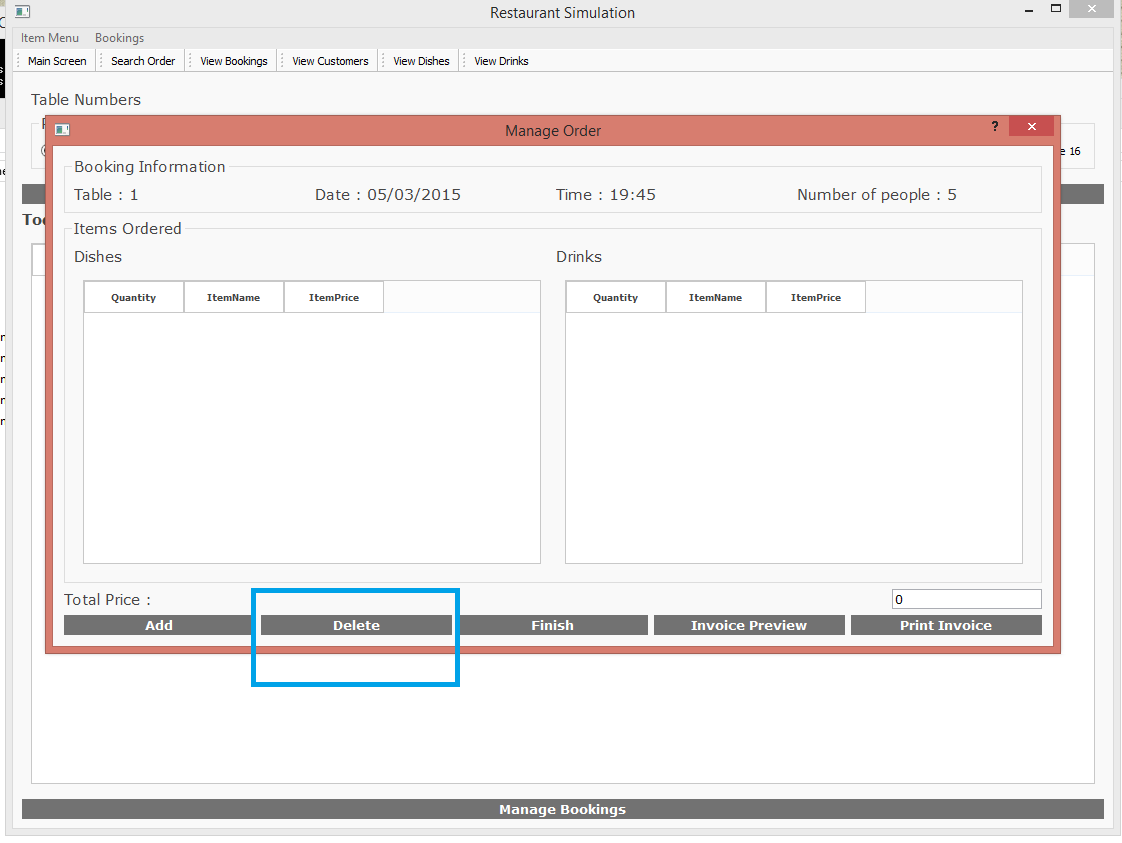
\includegraphics[height = 9cm]{./Manual/images/DeleteItemOrder1} 
    \caption{} \label{fig:deleteitemorder2}
\end{figure}

\begin{figure}[H]
    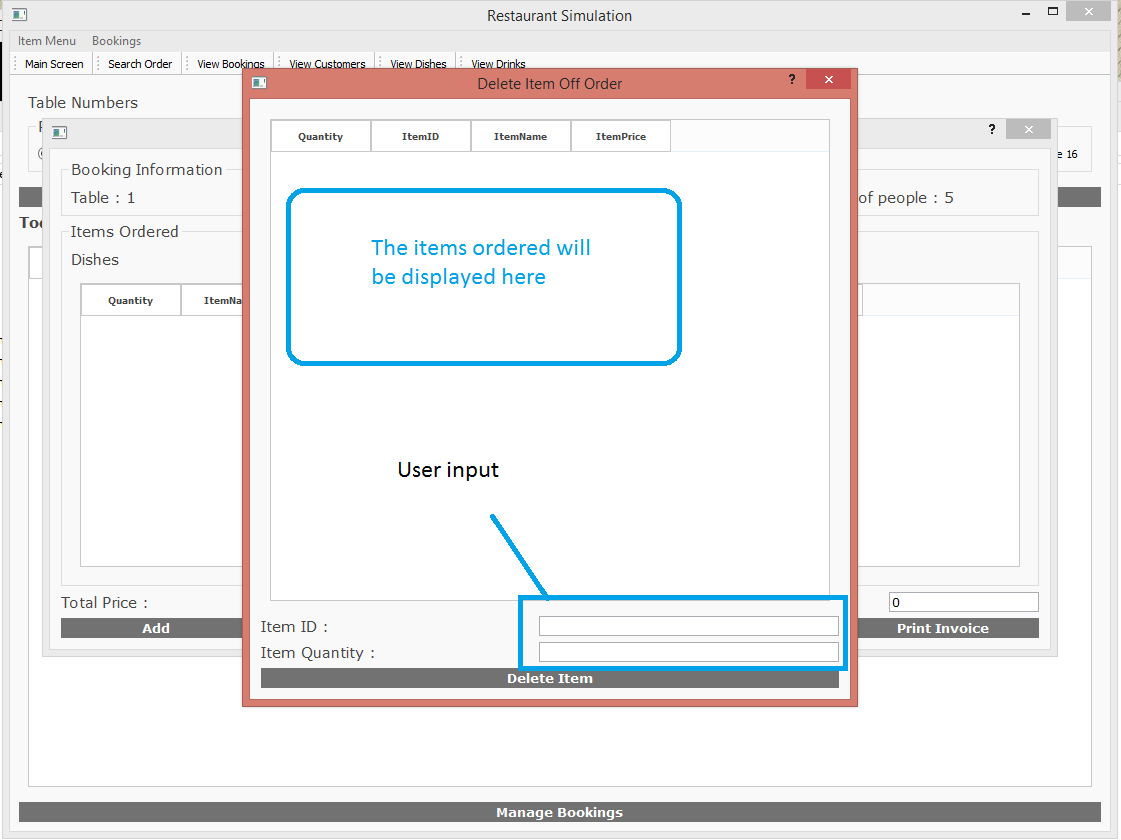
\includegraphics[height = 9cm]{./Manual/images/DeleteItemOrder2} 
    \caption{} \label{fig:deleteitemorder3}
\end{figure}

\subsection{How do I print an invoice?}
There are two ways to do so, through the manage order or from 'Search Order' on the tool bar.

\subsubsection{Manage Order method}
You will most likely find this method more convenient after a table has just finished with their meal .


\begin{figure}[H]
    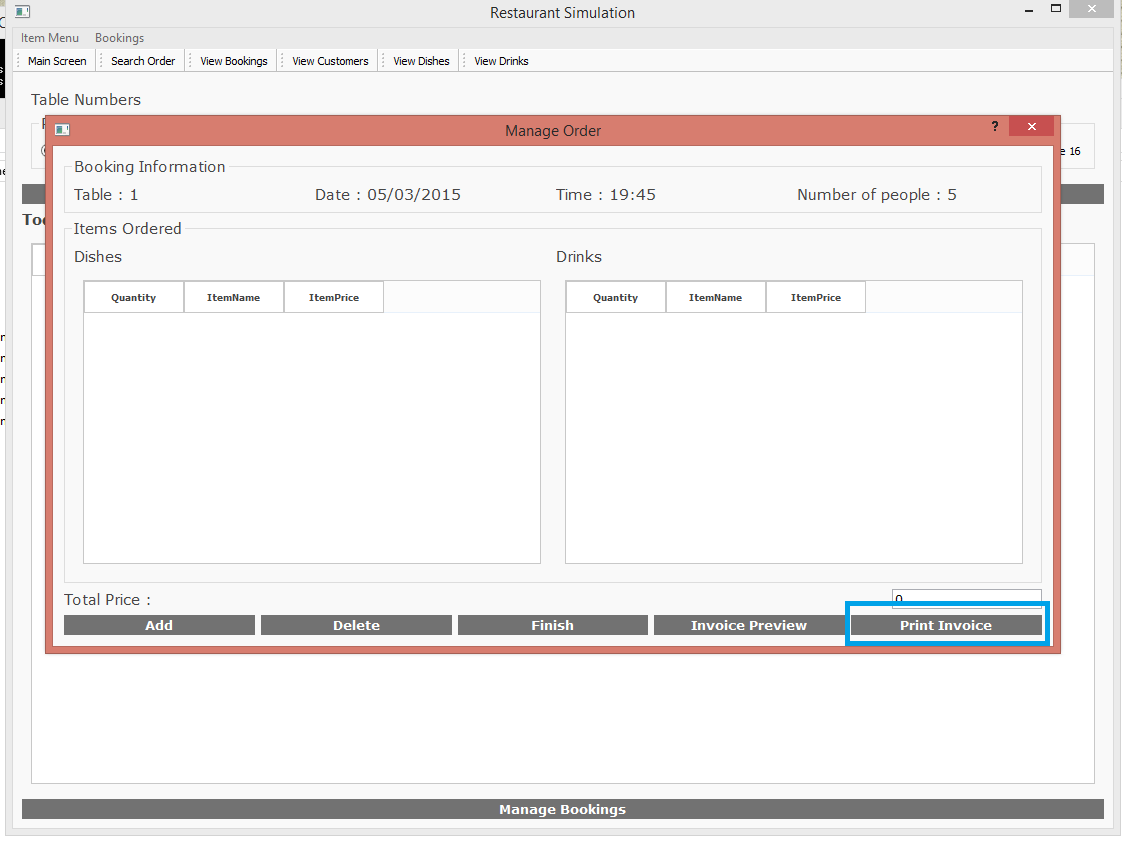
\includegraphics[height = 9cm]{./Manual/images/PrintInvoice1} 
    \caption{} \label{fig:printinvoice1}
\end{figure}

2. Click on 'Finish' after selecting the print options and the invoice should now begin to print
 
\begin{figure}[H]
    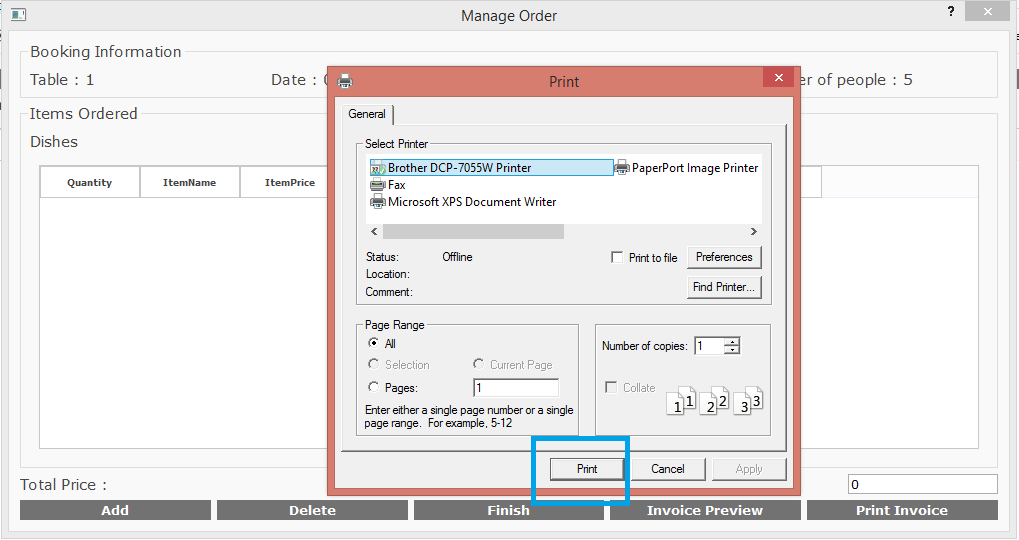
\includegraphics[height = 9cm]{./Manual/images/PrintInvoice2} 
    \caption{} \label{fig:printinvoice2}
\end{figure}

\subsubsection{Search Order method}
This method can be used to print invoices of any order that has been created.

\begin{figure}[H]
    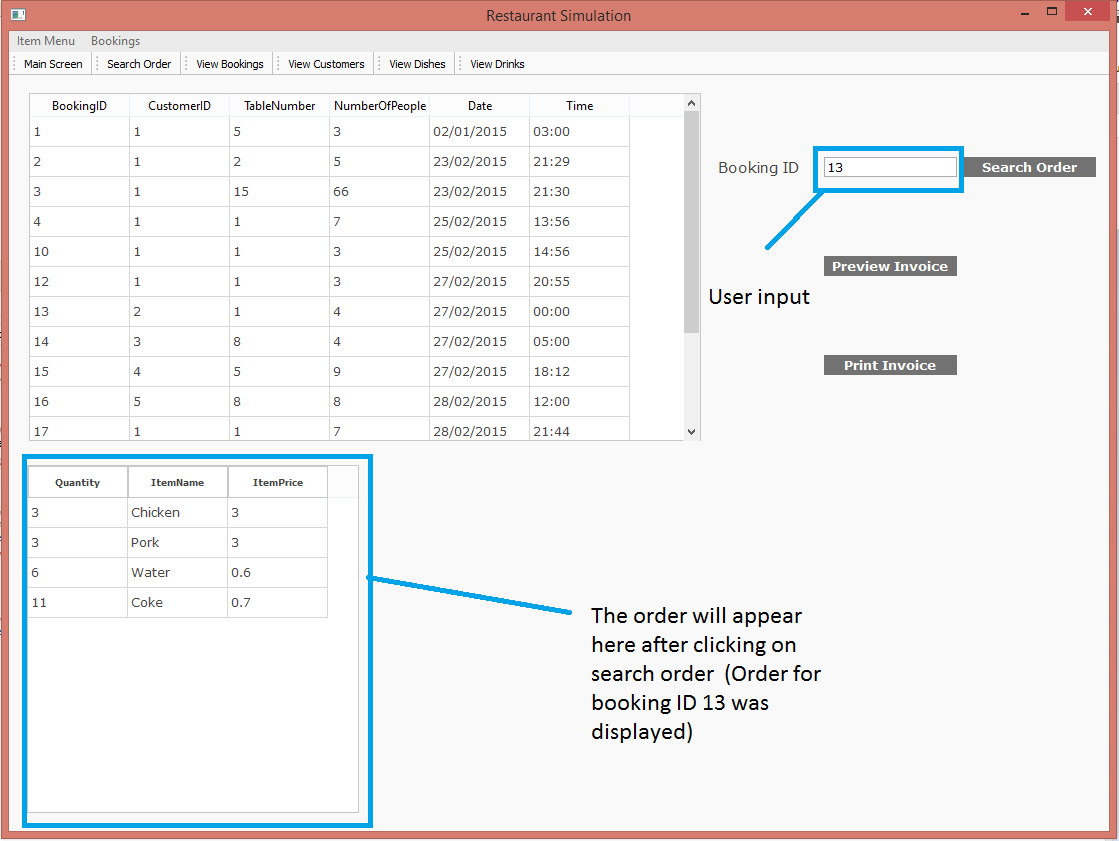
\includegraphics[height = 9cm]{./Manual/images/PrintInvoice3} 
    \caption{} \label{fig:printinvoice3}
\end{figure}

\begin{figure}[H]
    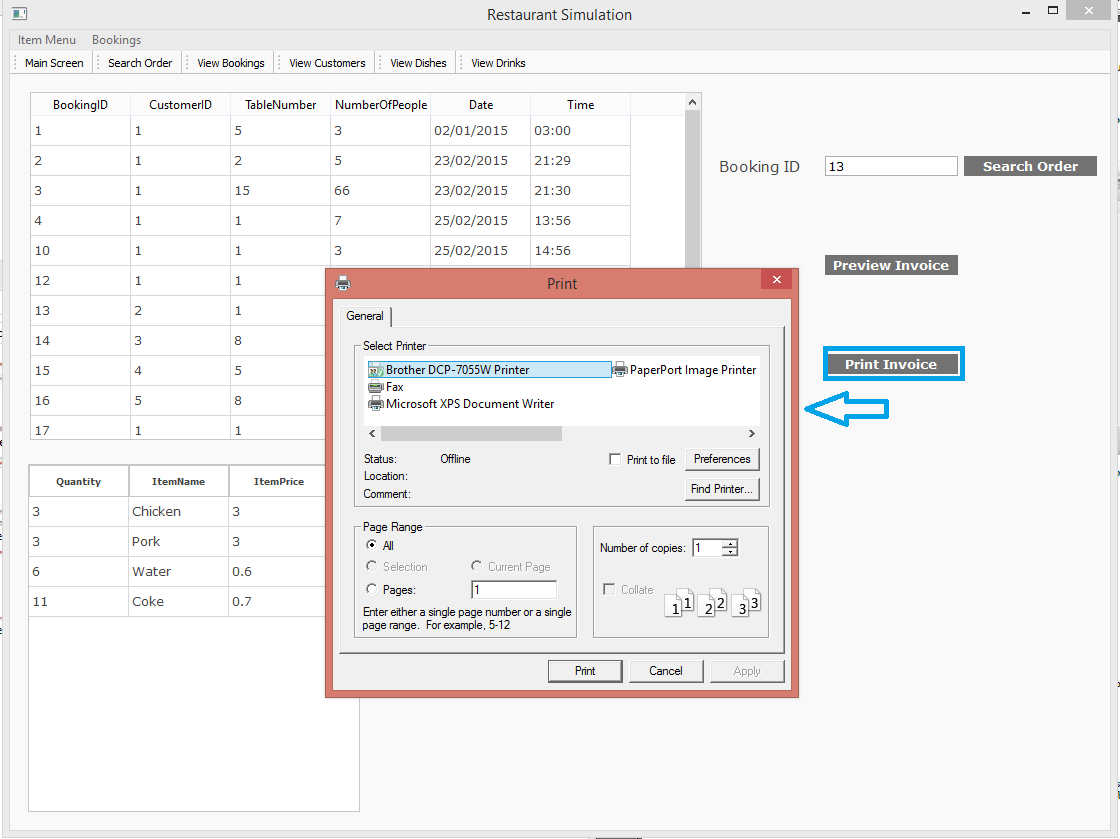
\includegraphics[height = 9cm]{./Manual/images/PrintInvoice4} 
    \caption{} \label{fig:printinvoice4}
\end{figure}


%need to do 'Finished' and invoice printing




\subsection{Saving}

The system saves automatically after executing a database query. For example, adding a booking or deleting an item off the menu.

\subsection{Limitations}

\section{Error Recovery}

%include as many subsections as necessary for each error
\subsection{Empty field error when trying to add an item}

Leaving empty fields will cause an error which is shown in the image below. \\


\begin{figure}[H]
    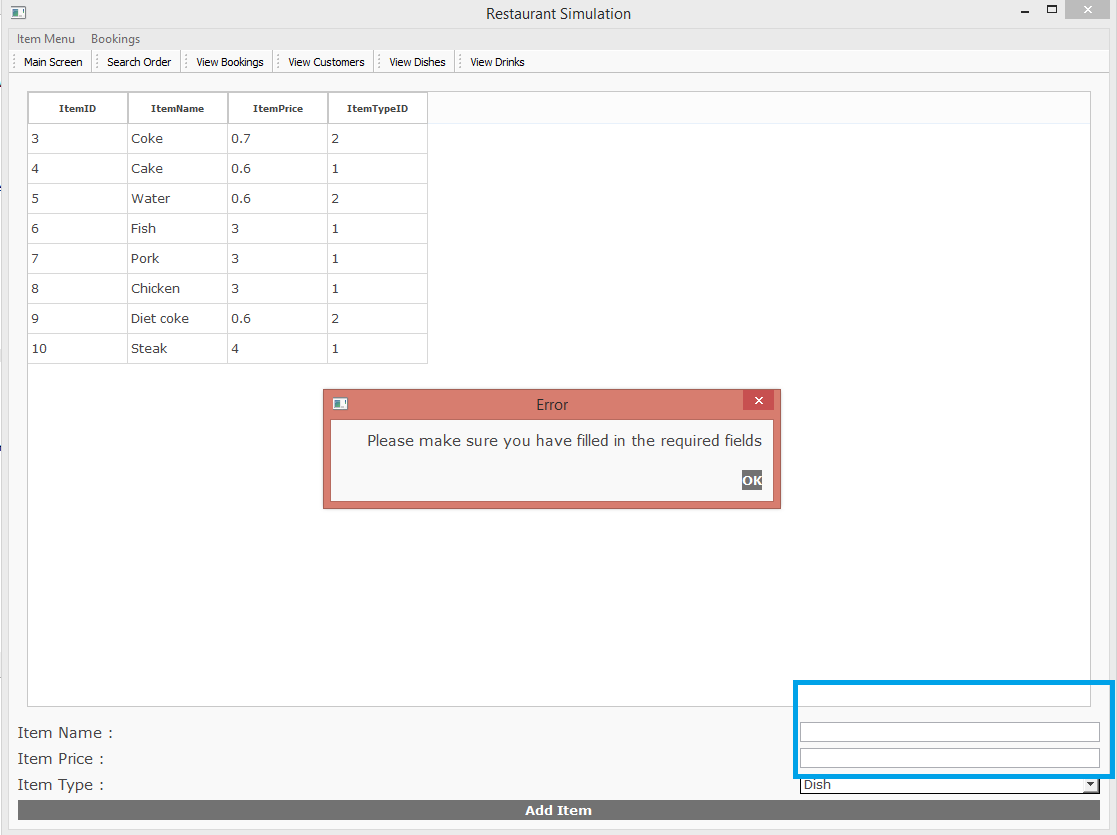
\includegraphics[height = 9cm]{./Manual/images/HamError1} 
    \caption{} \label{fig:hamerror1}
\end{figure}

As you can see in the image below, the item price field is empty which has caused the error to appear again.

\begin{figure}[H]
    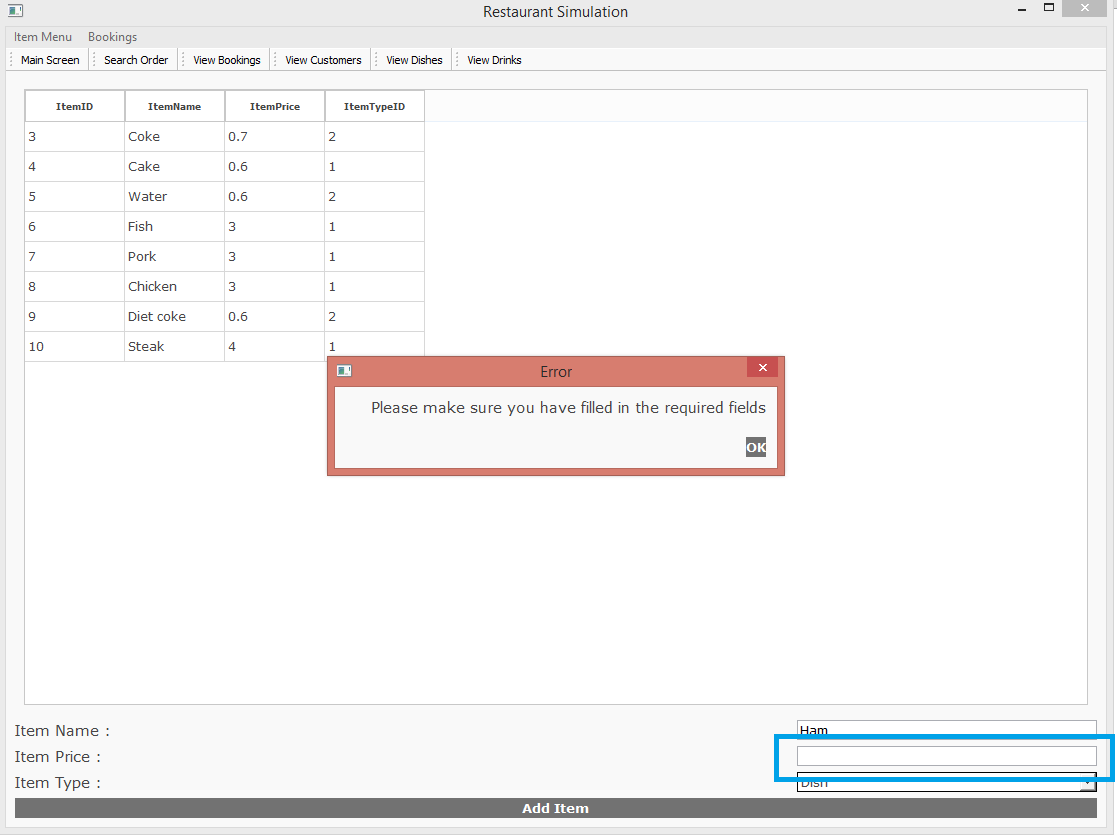
\includegraphics[height = 9cm]{./Manual/images/HamError2} 
    \caption{} \label{fig:hamerror2}
\end{figure}

To solve this, you would have to fill in the fields. As you can see in the image below, the new item has been added.

\begin{figure}[H]
    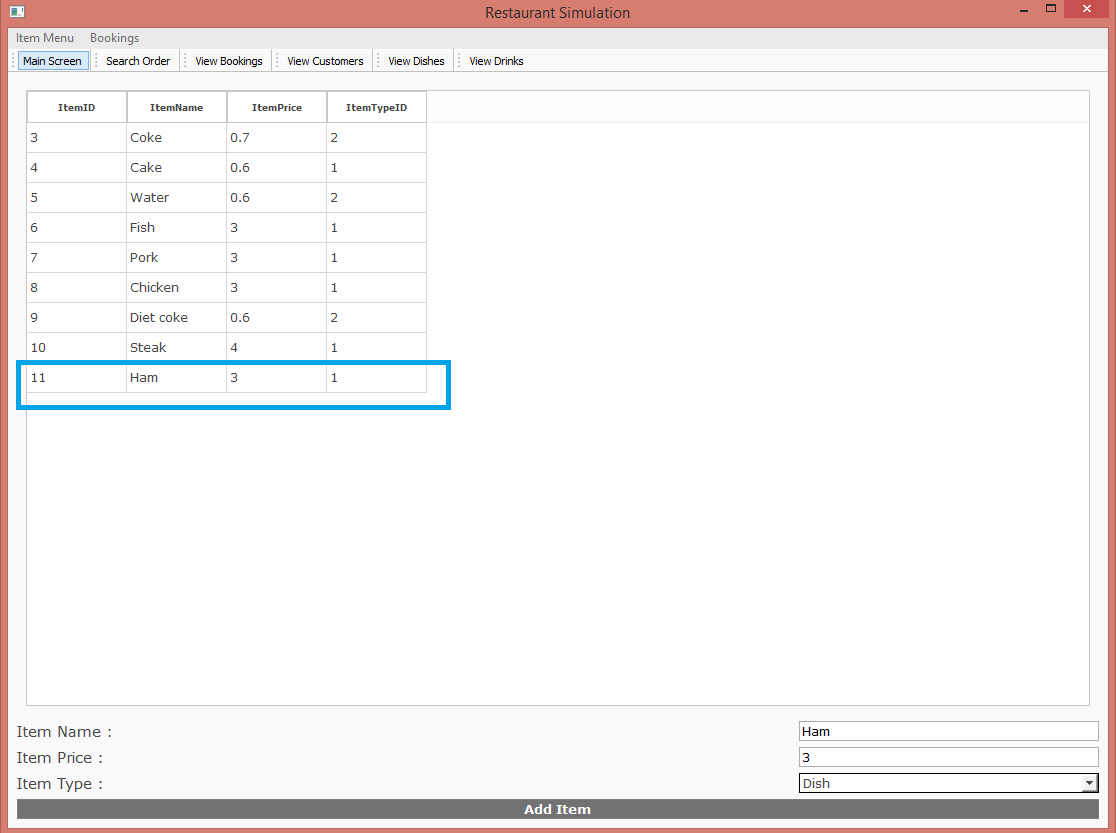
\includegraphics[height = 9cm]{./Manual/images/HamError3} 
    \caption{} \label{fig:hamerror3}
\end{figure}



\section{System Recovery}

\subsection{Backing-up Data}
The only data my client would need to back up is the database. To do this follow these steps:

1. Locate the system directory

2. Right-click on restaurant

3. Click on copy
\begin{figure}[H]
    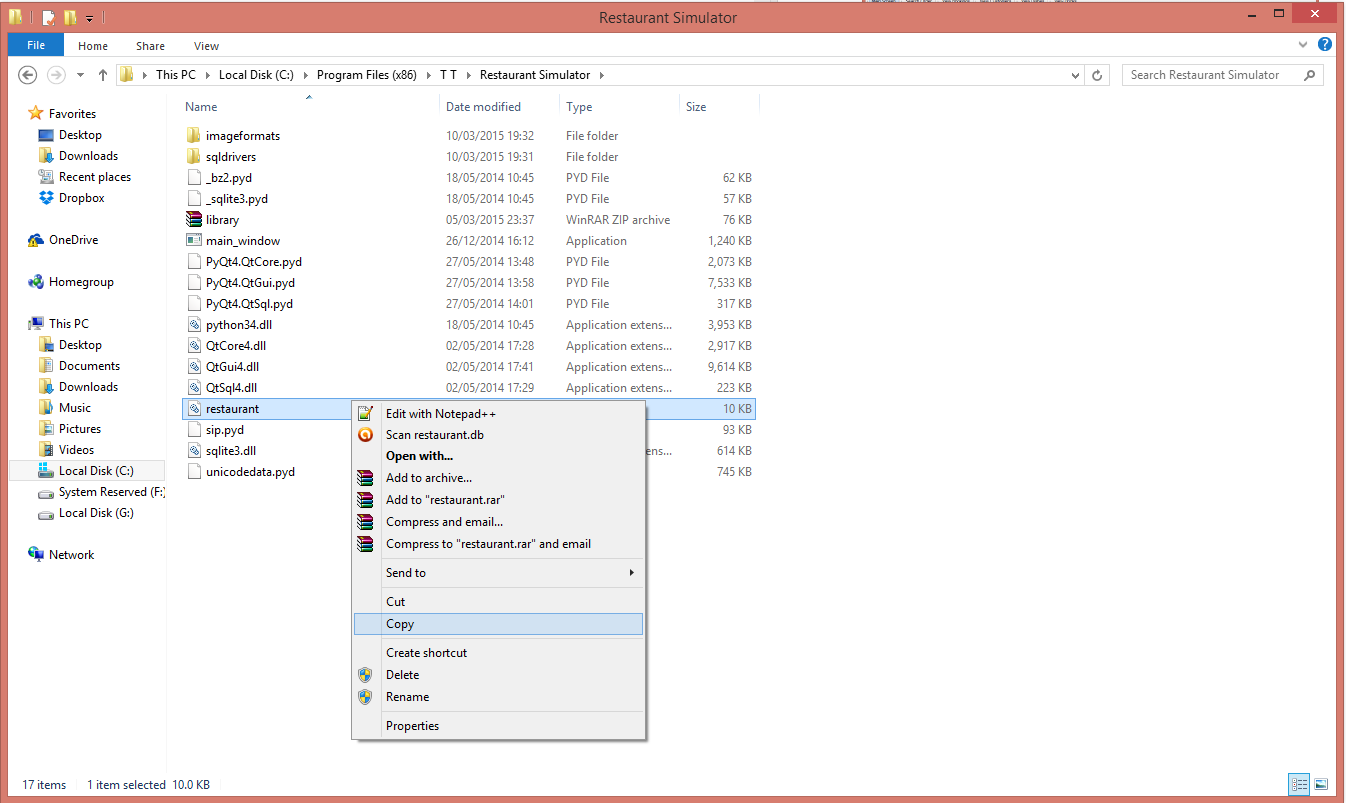
\includegraphics[height = 9cm]{./Manual/images/backup} 
    \caption{} \label{fig:backup}
\end{figure}

4. Go to the location where you want to back up the data ( I would recommend a USB)

5. Right - click and click on paste

\begin{figure}[H]
    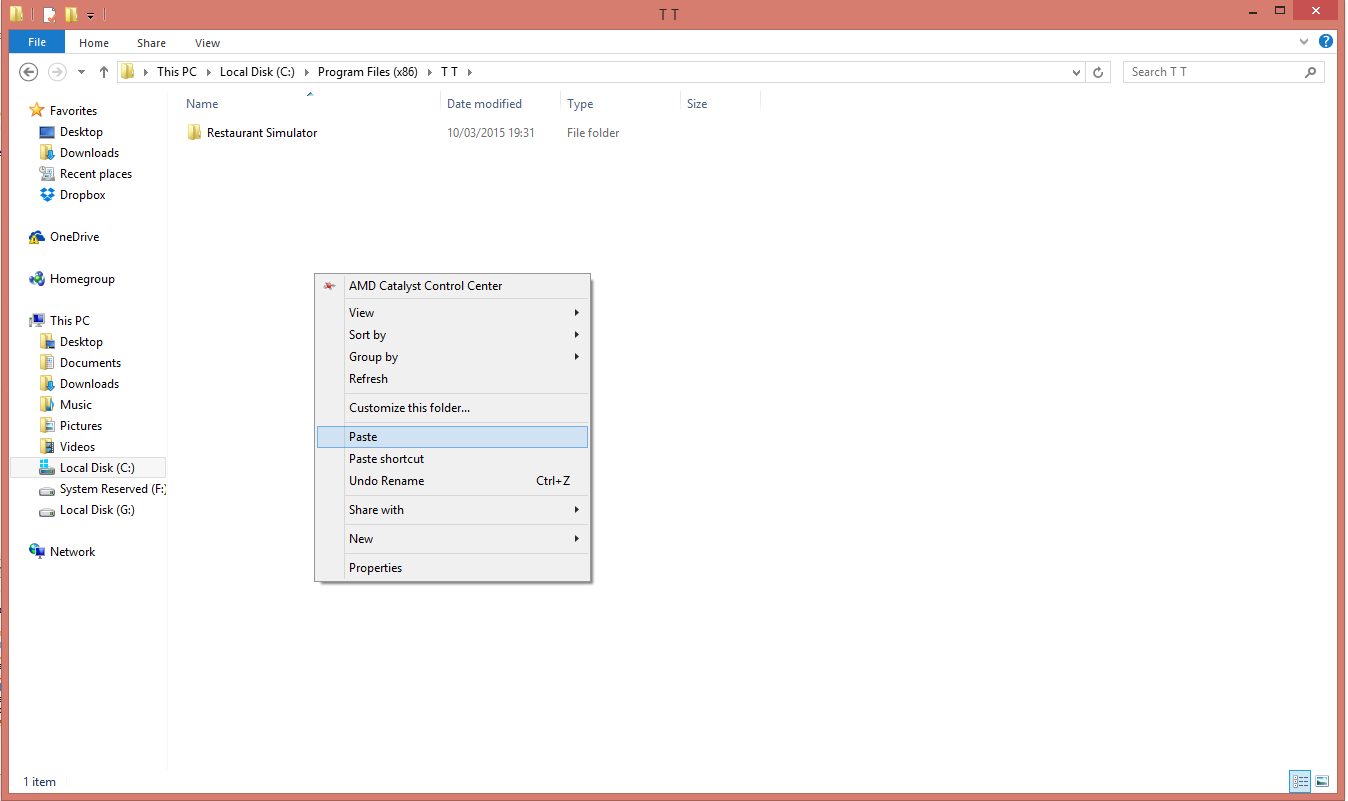
\includegraphics[height = 9cm]{./Manual/images/backup2} 
    \caption{} \label{fig:t}
\end{figure}

6. You have now backed-up the important file.
\begin{figure}[H]
    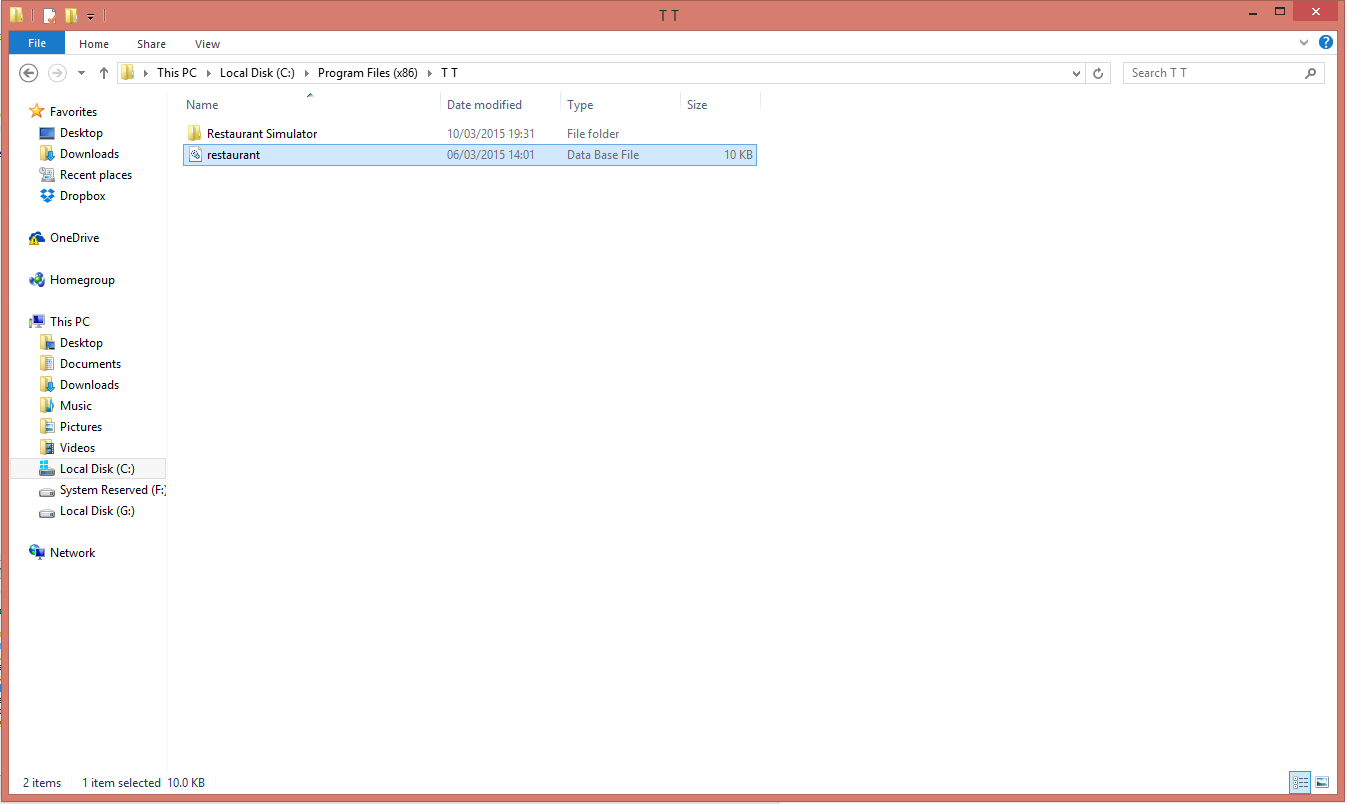
\includegraphics[height = 9cm]{./Manual/images/backup3} 
    \caption{} \label{fig:b}
\end{figure}

\subsection{Restoring Data}
To restore the data follow these steps:

1. Locate the file where you backed-up the data

2. Right-click on the restaurant db file

3. Click on Copy

\begin{figure}[H]
    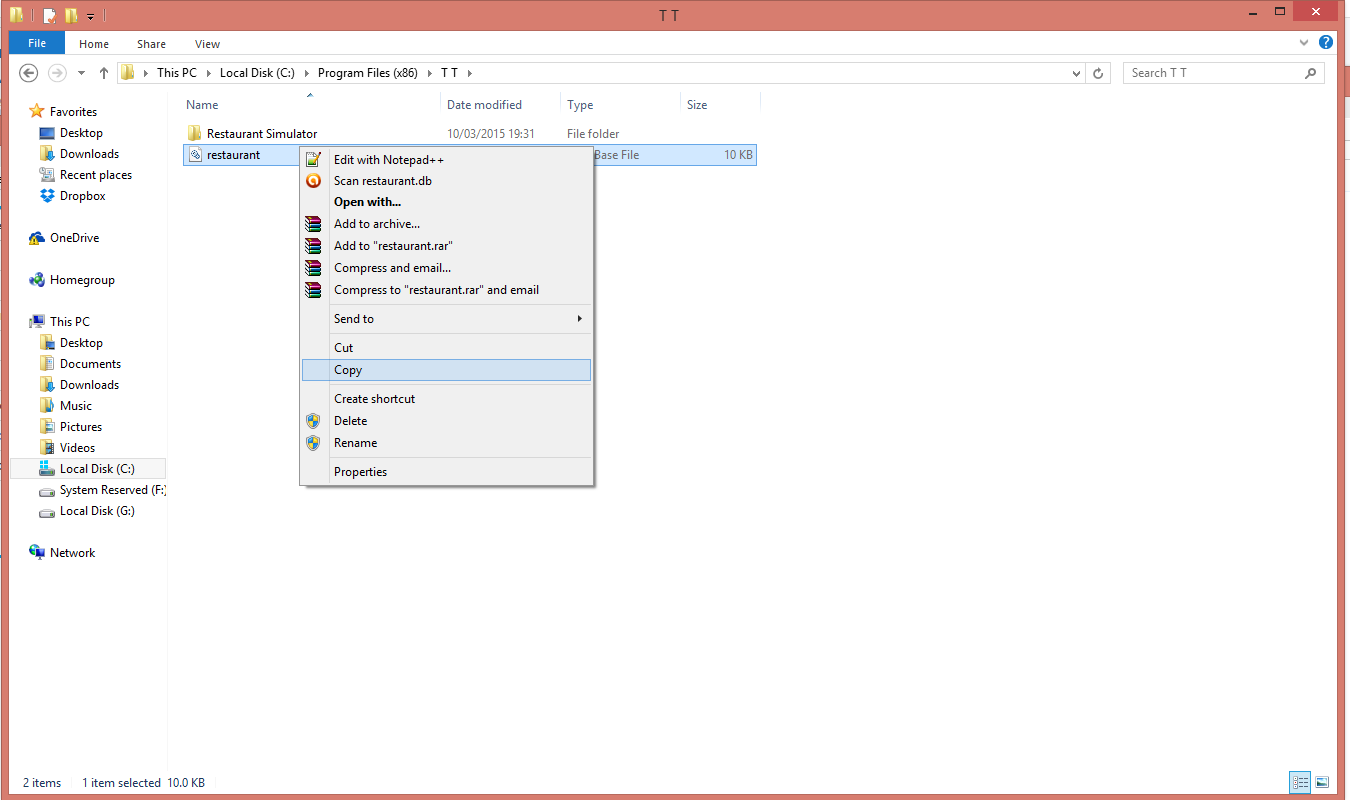
\includegraphics[height = 9cm]{./Manual/images/restore} 
    \caption{} \label{fig:hamerraor3}
\end{figure}

3. Go to the directory where the system was installed

4. Right-click and click on paste

\begin{figure}[H]
    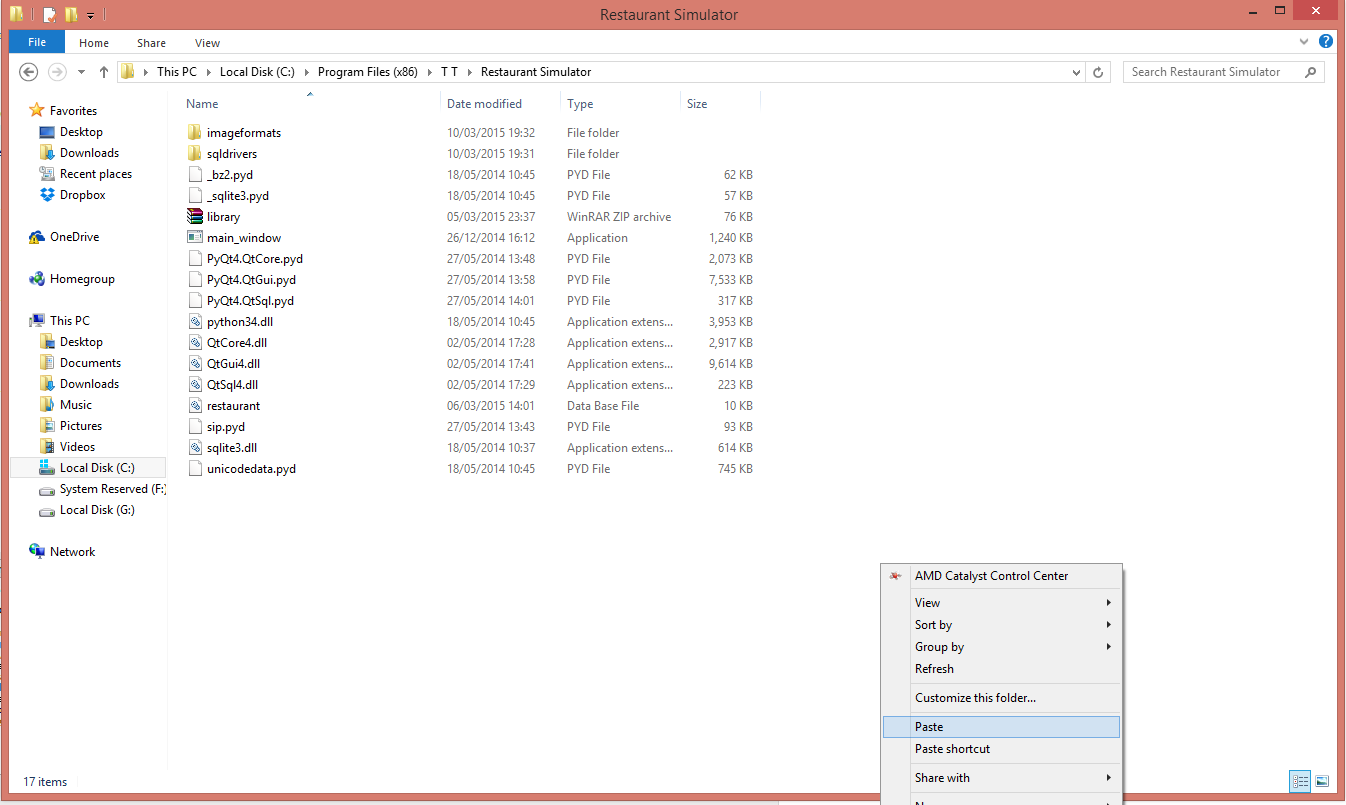
\includegraphics[height = 9cm]{./Manual/images/restore2} 
    \caption{} \label{fig:hamerfaraor3}
\end{figure}

5. Click on "Replace the file in the destination" if the message pops up

\begin{figure}[H]
    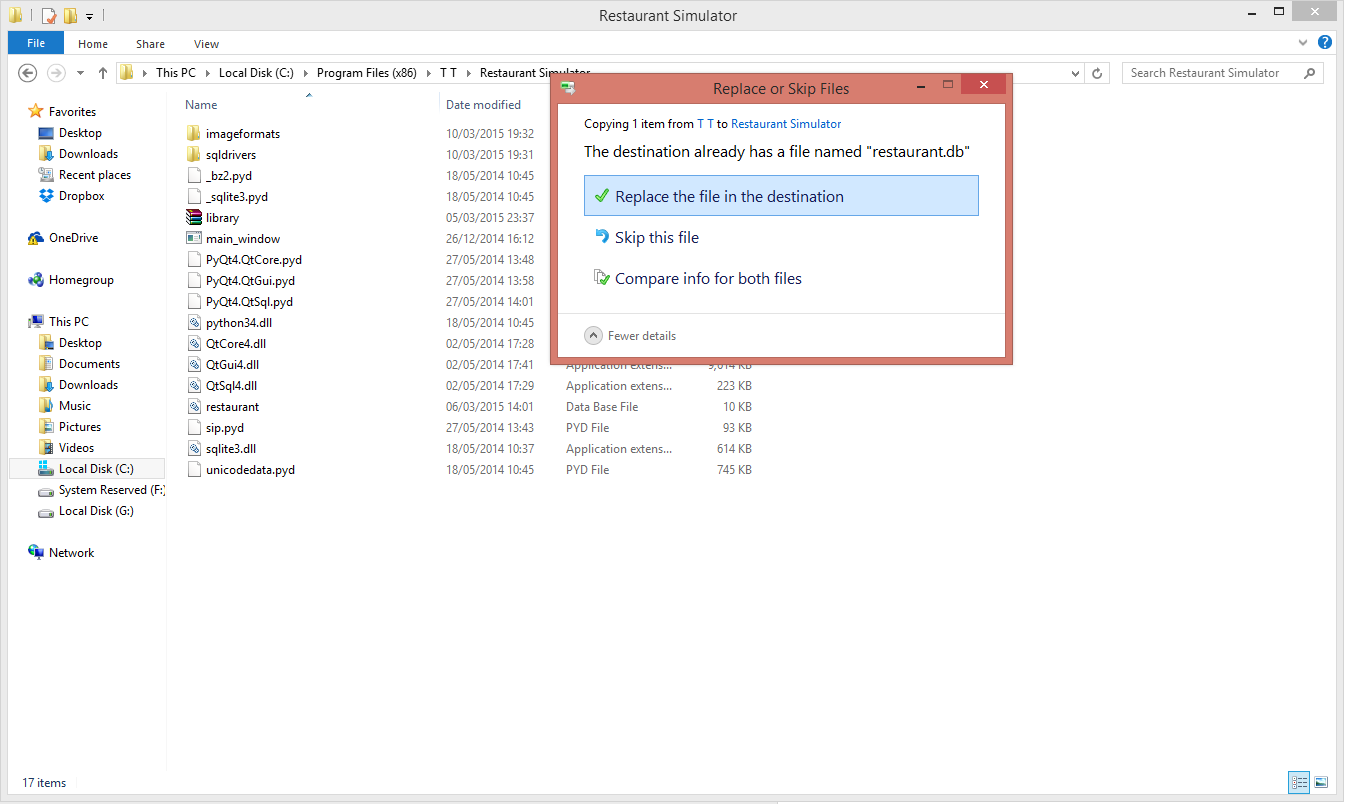
\includegraphics[height = 9cm]{./Manual/images/restore3} 
    \caption{} \label{fig:hamaerraor3}
\end{figure}

6. You have no backed-up the data

